\subsection{Stellar algebra of a locally compact group}

DEFINITION 9. --- Let G be a locally compact group and let A be the involutive Banach algebra of bounded measures on G admitting a density with respect to a Haar measure on G (Example 4 of I, p.~99). The enveloping stellar algebra of the involutive Banach algebra A is called the stellar algebra of G. It is denoted by Stell(G).

Note. --- Let \(\nu\) be a left Haar measure on G and let \(\Delta\) be its modulus. The map \(f \mapsto f \cdot \nu\) is an isometric isomorphism of the algebra \(\mathrm{L}^{1}(\mathrm{G}, \nu)\) onto A (loc. cit.). One can therefore also define Stell(G) as the enveloping stellar algebra of the normed involutive algebra \(\mathrm{L}^{1}(\mathrm{G}, \nu)\) .

Let G be a locally compact group and let \(\nu\) be a left Haar measure on G. For \(\mu \in \mathcal{M}^1 (\mathrm{G})\) and \(f\in \mathrm{L}^2 (\mathrm{G},\nu)\) , one has \(\mu *f\in \mathrm{L}^2 (\mathrm{G},\nu)\) (INT, VIII, §4, prop. 6). Let us then denote by \(\pmb{\gamma}(\mu)\) the endomorphism \(f\mapsto \mu *f\) of \(\mathrm{L}^2 (\mathrm{G},\nu)\) . The map \(\mu \mapsto \pmb{\gamma}(\mu)\) is a representation of the algebra \(\mathcal{M}^{1}(\mathrm{G})\) into the Banach algebra \(\mathcal{L}(\mathrm{L}^{2}(\mathrm{G},\nu))\) of continuous endomorphisms of \(\mathrm{L}^2 (\mathrm{G},\nu)\) (INT, VIII, §4, cor. of prop. 6). On the other hand, \(\gamma (\breve{\mu})\) is the transpose of the endomorphism \(\gamma (\mu)\) (INT, VIII, §4, no. 3, prop. 8). It follows that \(\gamma (\mu^{*})\) is the adjoint endomorphism of \(\gamma (\mu)\) , and therefore that the map \(\gamma \colon \mu \mapsto \gamma (\mu)\) is a morphism of involutive algebras from \(\mathcal{M}^{1}(\mathrm{G})\) into the stellar algebra \(\mathcal{L}(\mathrm{L}^{2}(\mathrm{G},\nu))\) , called the left regular representation of \(\mathcal{M}^{1}(\mathrm{G})\) in \(\mathrm{L}^2 (\mathrm{G},\nu)\) . According to INT, VIII, §4, no. 7, prop. 19, this representation is faithful.

Let \(j\) be the canonical map from \(\mathrm{L}^{1}(\mathrm{G},\nu)\) into \(\mathrm{Stell}(\mathrm{G})\) . By restriction to \(\mathrm{L}^{1}(\mathrm{G},\nu)\) , the regular representation \(\pmb{\gamma}\) defines an injective morphism of involutive algebras from \(\mathrm{L}^{1}(\mathrm{G},\nu)\) into \(\mathcal{L}(\mathrm{L}^{2}(\mathrm{G},\nu))\) , called the left regular representation of \(\mathrm{L}^{1}(\mathrm{G})\) in \(\mathrm{L}^{2}(\mathrm{G})\) . According to prop. 20, there exists a unique morphism \(\pmb{\gamma}'\colon \mathrm{Stell}(\mathrm{G})\to \mathcal{L}(\mathrm{L}^{2}(\mathrm{G},\nu))\) such that \(\pmb{\gamma} = \pmb{\gamma}'\circ j\) . We say that \(\pmb{\gamma}'\) is the left regular representation of \(\mathrm{Stell}(\mathrm{G})\) in \(\mathrm{L}^{2}(\mathrm{G},\nu)\) . By abuse of notation, we will still denote it by

\[
\boldsymbol {\gamma} ^ {\prime} (\varphi) (f) = \varphi * f\tag{7}
\]

for \(f\in \mathrm{L}^2 (\mathrm{G},\nu)\) and \(\varphi \in \mathrm{Stell}(\mathrm{G})\) . We have

\[
\| \varphi * f \| _ {2} \leqslant \| \varphi \| _ {*} \| f \| _ {2}.\tag{8}
\]

Remark. --- In general, the left regular representation \(\gamma'\) of Stell(G) in \(L^{2}(G,\nu)\) is not faithful. One can show that it is faithful if and only if there exists a positive linear form f on \(\mathrm{L}_{\mathbf{R}}^{\infty}(\mathrm{G})\) such that \(f(1)=1\) and \(f(\boldsymbol{\gamma}(g)x)=f(x)\) for all \((g,x)\in\mathrm{G}\times\mathrm{G}\) (we then say that the group G is amenable, cf.~EVT, IV, p.~73, exercise 4).

PROPOSITION 22. --- The canonical map j from \(\mathrm{L}^{1}(\mathrm{G},\nu)\) into Stell(G) is injective and has dense image.

The image of \(j\) is dense by definition of the enveloping stellar algebra of a normed involutive algebra. Since the left regular representation \(\gamma\) is faithful, the injectivity of \(j\) follows from the equality \(\gamma = \gamma' \circ j\) .

COROLLARY. --- The algebra \(\mathrm{L}^{1}(\mathrm{G},\nu)\) is radical-free.

This follows from prop. 21 of I, p.~125 and from prop. 22.

Thus one can identify \(\mathrm{L}^{1}(\mathrm{G},\nu)\) with a dense involutive subalgebra of \(\mathrm{Stell}(\mathrm{G})\) , and the canonical injection of \(\mathrm{L}^{1}(\mathrm{G},\nu)\) into \(\mathrm{Stell}(\mathrm{G})\) is then continuous.

Suppose now that the group G is unimodular (INT, VII, §1, no. 3, def. 3). One can then repeat the same arguments starting from the right regular representation \((f,\mu)\mapsto\boldsymbol{\delta}(\mu)(f)=f*\breve{\mu}\) of \(\mathrm{L}^{2}(\mathrm{G},\nu)\times\mathcal{M}^{1}(\mathrm{G})\) into \(\mathrm{L}^{2}(\mathrm{G},\nu)\) . We then define a morphism \(\delta^{\prime}\) of \(\operatorname{Stell}(\mathrm{G})\) into \(\mathcal{L}(\mathrm{L}^{2}(\mathrm{G},\nu))\) such that \(\delta=\delta^{\prime}\circ j\) , and define \(\boldsymbol{\delta}^{\prime}(\varphi)(f)=f*\varphi\) for \(f\in\mathrm{L}^{2}(\mathrm{G},\nu)\) and \(\varphi\in\operatorname{Stell}(\mathrm{G})\) .

For \(\varphi, \psi \in \text{Stell}(G)\) , one has \(\boldsymbol{\delta}'(\psi) \circ \boldsymbol{\gamma}'(\varphi) = \boldsymbol{\gamma}'(\psi) \circ \boldsymbol{\delta}'(\varphi)\) , that is,

\[
(\varphi * f) * \psi = \varphi * (f * \psi)\tag{9}
\]

for all \(f \in \mathrm{L}^{2}(\mathrm{G}, \nu)\) . Indeed, this formula is true for \(\varphi, \psi \in \mathrm{L}^{1}(\mathrm{G}, \nu)\) , and the maps \((\varphi, \psi) \mapsto (\varphi * f) * \psi\) and \((\varphi, \psi) \mapsto \varphi * (f * \psi)\) are continuous bilinear maps from \(\operatorname{Stell}(\mathrm{G}) \times \operatorname{Stell}(\mathrm{G})\) into \(\mathrm{L}^{2}(\mathrm{G}, \nu)\) .

\section{SPECTRUM OF ENDOMORPHISMS OF BANACH SPACES}

Unless stated otherwise, the vector spaces considered in this paragraph are vector spaces over C. We denote by \(1_{E}\) the identity map of a vector space E. An endomorphism of a topological vector space E is a continuous linear map from E to E.

Let E be a topological vector space and u an endomorphism of E. If F is a subspace of E stable under u, we shall say that the endomorphism of F deduced from u by restriction is the endomorphism of F deduced from u. We denote it by \(u|F\) .

\subsection{Spectrum of an endomorphism}

DEFINITION 1. --- Let E be a topological vector space and let u be an endomorphism of E. We call the spectrum of u, and denote by Sp(u), the spectrum of u relative to the unital algebra \(\mathcal{L}(\mathrm{E})\) .

Let E be a topological vector space and let \(u \in \mathcal{L}(\mathrm{E})\) . The spectrum of u is the set of complex numbers \(\lambda\) such that \(u - \lambda1_{E}\) is not an automorphism of E. If E is metrizable and complete, it is also the set of complex numbers \(\lambda\) such that \(u - \lambda1_{E}\) is not bijective (EVT, I, p.~19, cor. 1).

Every eigenvalue of u belongs to the spectrum of u, but the converse is false in general.

In the rest of this paragraph, we shall restrict ourselves to studying the notion of spectrum in the case where E is a Banach space.

Lemma 1. --- Let E be a Banach space and let u be an endomorphism of E. Let \((\mathrm{E}_{i})_{i\in\mathrm{I}}\) be a finite family of closed subspaces of E, stable under u, such that \(E = \bigoplus_{i\in I} E_{i}\) . For every \(i \in I\) , let \(u_{i}\) be the endomorphism of \(E_{i}\) induced by u. We have \(\mathrm{Sp}(u) = \bigcup_{i\in I} \mathrm{Sp}(u_{i})\) , and for every \(f \in \mathcal{O}(\mathrm{Sp}(u))\) , the endomorphism \(f(u)\) stabilizes the spaces \(E_{i}\) , and \(f(u)\) coincides with \(f(u_{i})\) on \(E_{i}\) .

The endomorphism \(u\) is an isomorphism if and only if \(u_i\) is an isomorphism for every \(i \in \mathrm{I}\) . Applying this property to \(u - \lambda 1_{\mathrm{E}}\) , one deduces that \(\operatorname{Sp}(u)\) is the union of the sets \(\operatorname{Sp}(u_i)\) for \(i \in \mathrm{I}\) .

Let \(f \in \mathcal{O}(\mathrm{Sp}(u))\) . The endomorphism \(f(u)\) of E belongs to the bicommutant of \(u\) in \(\mathcal{L}(\mathrm{E})\) (theorem 5 of I, p.~74), hence it commutes with the projections \(p_i\) . It then stabilizes the spaces \(\mathrm{E}_i\) . Consider the continuous unital morphism \(\varpi\) of the product algebra \(\prod_{i \in \mathrm{I}} \mathcal{L}(\mathrm{E}_i)\) into \(\mathcal{L}(\mathrm{E})\) defined by \((v_i)_{i \in \mathrm{I}} \mapsto \bigoplus_i v_i\) . It maps the family \((u_i)\) to \(u\) . Proposition 7 of I, p.~75 then implies that \(\mathrm{Sp}(u) \subset \bigcup_{i \in \mathrm{I}} \mathrm{Sp}(u_i)\) and

\[
f (u) = f (\varpi ((u _ {i}) _ {i \in \mathrm{I}})) = \varpi ((f (u _ {i})) _ {i \in \mathrm{I}}) = \bigoplus_ {i \in \mathrm{I}} f (u _ {i}),
\]

which concludes the proof of the lemma.

PROPOSITION 1. --- Let E be a complex Banach space and let u be an endomorphism of E. Let \(\lambda \in \mathbf{C}\) and \(f \in \mathcal{O}(\mathrm{Sp}(u))\) . We have

\[
\operatorname{Ker} (u - \lambda 1 _ {\mathrm{E}}) \subset \operatorname{Ker} (f (u) - f (\lambda) 1 _ {\mathrm{E}}).
\]

Let \(x \in E\) be nonzero. The set A of \(v \in \mathcal{L}(E)\) such that \(x\) is an eigenvector of \(v\) is a unital subalgebra of \(\mathcal{L}(E)\) .

The algebra A is full: if \(v \in A\) is invertible in \(\mathcal{L}(\mathrm{E})\) and if x is an eigenvector of v for the eigenvalue \(\lambda\) , then \(\lambda \neq 0\) and \(v^{-1}(x) = \lambda^{-1}x\) which proves that \(v^{-1} \in A\) .

The algebra A is closed in \(\mathcal{L}(\mathrm{E})\) . Indeed, if \((v_n)_{n\in \mathbf{N}}\) is a sequence in A such that \(v_{n}\) converges to \(v\in \mathcal{L}(\mathrm{E})\) , the sequence \((\lambda_{n})_{n\in \mathbf{N}}\) such that \(v_{n}(x) = \lambda_{n}x\) is bounded, hence admits a subsequence converging to a complex number \(\mu\) , so that \(v(x) = \mu x\) .

Suppose that \(x\) is an eigenvector of \(u\) and that \(u(x) = \lambda x\) . The algebra A contains \(u\) , hence contains the closed unital full subalgebra B generated by \(u\) , which is commutative. The map \(\chi \colon \mathrm{B} \to \mathbf{C}\) which associates with \(v\) the eigenvalue of \(v\) relative to \(x\) is a character of B such that \(\chi(u) = \lambda\) . For every \(f \in \mathcal{O}(\mathrm{Sp}(u))\) , one has \(f(u) \in \mathrm{B}\) and \(\chi(f(u)) = f(\chi(u)) = f(\lambda)\) by prop. 7 of I, p.~75, whence the proposition.

\subsection{Spectral projectors}

Let E be a Banach space. We denote by A the unital Banach algebra \(\mathcal{L}(\mathrm{E})\) of endomorphisms of E. Let \(u\in \mathrm{A}\) .

Let H be a subset of \(\mathrm{Sp}(u)\) which is open and closed in \(\mathrm{Sp}(u)\) ; denote by K its complement in \(\mathrm{Sp}(u)\) .

The idempotent element associated with \(u\) and H (no. 12 of I, p.~81) is a continuous projector of E, called the spectral projector associated with \(u\) and H; it is denoted \(e_{\mathrm{H}}(u)\) , or simply \(e_{\mathrm{H}}\) . Its image is called the spectral subspace of E associated with \(u\) and H, and is denoted \(\mathrm{E_H}(u)\) , or simply \(\mathrm{E_H}\) . Its kernel is \(\mathrm{E_K}(u)\) , and is also denoted \(\widetilde{\mathrm{E}}_{\mathrm{H}}(u)\) , or simply \(\widetilde{\mathrm{E}}_{\mathrm{H}}\) . The space E is the topological direct sum of the closed subspaces \(\mathrm{E_H}\) and \(\mathrm{E_K}\) . The condition \(\mathrm{E_H} = 0\) is equivalent to \(e_{\mathrm{H}} = 0\) , that is, to the indicator function \(f_{\mathrm{H}}\) of H on \(\mathrm{Sp}(u)\) being the zero function, and hence to \(\mathrm{H} = \varnothing\) .

Every endomorphism v of E that commutes with u also commutes with \(e_{\mathrm{H}}(u)\) (th. 5 of I, p.~74), hence stabilizes \(E_{H}\) and \(E_{K}\) . In particular, the endomorphism u leaves the subspaces \(E_{H}\) and \(E_{K}\) stable. The space \(E_{K}\) is the only topological supplement of \(E_{H}\) in E that is stable under u.

The unital algebra \(A_{H} = e_{H}Ae_{H}\) (loc. cit.) is the subalgebra of A consisting of the endomorphisms of E that leave \(E_{H}\) stable and that vanish on \(E_{K}\) . For every \(v \in A_{H}\) , we denote by \(v|E_{H}\) the endomorphism of \(E_{H}\) deduced from v. The map \(v \mapsto v|E_{H}\) is an isomorphism from \(A_{H}\) onto \(\mathcal{L}(E_{\mathrm{H}})\) . In particular, we have \(\mathrm{Sp}(u|E_{\mathrm{H}}) = \mathrm{Sp}_{\mathrm{A}_{\mathrm{H}}} (u|E_{\mathrm{H}}) = H\) and \(\mathrm{Sp}_{\mathrm{A}_{\mathrm{K}}} (u|E_{\mathrm{K}}) = K\) by formula (18) of I, p.~82.

PROPOSITION 2. --- Let E be a Banach space and let u be an endomorphism of E. Let \(E_{1}\) and \(E_{2}\) be closed subspaces of E stable under u such that \(E = E_{1} \oplus E_{2}\) . Suppose that the endomorphisms \(u_{1}\) and \(u_{2}\) of \(E_{1}\) and \(E_{2}\) deduced from u have disjoint spectra \(H_{1} = \mathrm{Sp}(u_{1})\)

and \(\mathrm{H}_2 = \mathrm{Sp}(u_2)\) . Then \(\mathrm{Sp}(u) = \mathrm{H}_1 \cup \mathrm{H}_2\) and \(e_{\mathrm{H}_1}(u)\) is the projector with image \(\mathrm{E}_1\) and kernel \(\mathrm{E}_2\) . In particular, we have \(\mathrm{E}_{\mathrm{H}_1} = \mathrm{E}_1\) and \(\mathrm{E}_{\mathrm{H}_2} = \mathrm{E}_2\) .

We have \(\mathrm{Sp}(u)=\mathrm{H}_{1}\cup\mathrm{H}_{2}\) (I, p.~128, lemma 1). Since the sets \(H_{1}\) and \(H_{2}\) are compact, they are open and closed in \(\mathrm{Sp}(u)\) . For every holomorphic function f in a neighborhood of \(\mathrm{Sp}(u)\) , the endomorphism \(f(u)\) stabilizes \(E_{1}\) and \(E_{2}\) and coincides on \(E_{1}\) with \(f(u_{1})\) and on \(E_{2}\) with \(f(u_{2})\) (loc. cit.). Take in particular for f the germ of a holomorphic function \(f_{H_{1}}\) which equals 1 in a neighborhood of \(H_{1}\) and 0 in a neighborhood of \(H_{2}\) (cf. no. 12 of I, p. 81); then \(f_{\mathrm{H}_{1}}(u_{1})\) is the identity map of \(E_{1}\) since \(f_{H_{1}}=1\) in a neighborhood of \(\mathrm{H}_{1}=\mathrm{Sp}(u_{1})\) , and \(f_{\mathrm{H}_{1}}(u_{2})\) is zero since \(f_{H_{1}}=0\) in a neighborhood of \(H_{2}\) . Therefore \(e_{\mathrm{H}_{1}}(u)=f_{\mathrm{H}_{1}}(u)\) is the projector with image \(E_{1}\) and kernel \(E_{2}\) , and we therefore have \(E_{1}=E_{H_{1}}\) and \(E_{2}=E_{H_{2}}\) .

Let E be a Banach space and u an endomorphism of E. Let \((\mathrm{H}_{i})_{i\in\mathrm{I}}\) be a finite family of open and closed subsets of \(\mathrm{Sp}(u)\) , pairwise disjoint, and let H be their union. Relations (15) and (16) of I, p.~81 imply the following assertions:

\begin{enumerate}
\def\labelenumi{\alph{enumi})}
\item
  The family of projectors \((e_{\mathrm{H}_{i}}(u))_{i\in\mathrm{I}}\) is orthogonal (that is, \(e_{\mathrm{H}_{i}}(u)e_{\mathrm{H}_{j}}(u)=0\) for all \((i,j)\) in I² such that \(i\neq j\) , cf.~A, II, p.~18, def. 7) and its sum is \(e_{\mathrm{H}}(u)\) ;
\item
  The vector space \(E_{H}\) is the topological direct sum of the family \((\mathrm{E}_{\mathrm{H}_{i}})_{i\in\mathrm{I}}\) ;
\item
  For every \(j \in \mathrm{I}\) , one has \(\mathrm{E}_{\mathrm{Sp}(u) - \mathrm{H}_j} = \mathrm{E}_{\mathrm{Sp}(u) - \mathrm{H}} \oplus \bigoplus_{i \neq j} \mathrm{E}_{\mathrm{H}_i}\) ;
\item
  The vector space \(\mathrm{E}_{\mathrm{Sp}(u)-\mathrm{H}}\) is the intersection of the family \((\mathrm{E}_{\mathrm{Sp}(u)-\mathrm{H}_i})_{i\in\mathrm{I}}\) .
\end{enumerate}

When \(\mathrm{H} = \mathrm{Sp}(u)\) , the topological direct sum decomposition \(\bigoplus_{i \in I} E_{H_i}\) of E is called the spectral decomposition of E associated with u and the finite partition \((\mathrm{H}_i)_{i \in I}\) of \(\mathrm{Sp}(u)\) .

Let \(f\) be an element of \(\mathcal{O}(\mathrm{Sp}(u))\) . The spectrum of the endomorphism \(f(u)\) of E is the image under \(f\) of the spectrum of \(u\) (I, p.~75, prop. 8). Let L be an open and closed subset of \(\mathrm{Sp}(f(u))\) . The set H of elements \(\lambda \in \mathrm{Sp}(u)\) such that \(f(\lambda)\) belongs to L is open and closed in \(\mathrm{Sp}(u)\) , and we have \(e_{\mathrm{L}}(f(u)) = e_{\mathrm{H}}(u)\) since \(f_{\mathrm{L}} \circ f = f_{\mathrm{H}}\) in \(\mathcal{O}(\mathrm{Sp}(u))\) (loc. cit.).

\subsection{Isolated points of the spectrum}

Let E be a Banach space and let u be an endomorphism of E. Let \(\lambda\in C\) be an isolated point of \(\mathrm{Sp}(u)\) . We then denote by \(\mathrm{E}_{\lambda}(u)=\mathrm{E}_{\{\lambda\}}(u)\) and \(e_{\lambda}(u)\) the spectral projector with image \(\mathrm{E}_{\lambda}(u)\) associated with u and \(\{\lambda\}\) .

We also denote by \(\widetilde{\mathrm{E}}_{\lambda}(u) = \mathrm{E}_{\mathrm{Sp}(u) - \{\lambda\}}(u)\) . The spectrum of the endomorphism of \(\widetilde{\mathrm{E}}_{\lambda}(u)\) induced by \(u\) is \(\mathrm{Sp}(u) - \{\lambda\}\) ; in particular, \(u - \lambda 1_{\mathrm{E}}\) induces an automorphism of \(\widetilde{\mathrm{E}}_{\lambda}(u)\) .

The space \(\mathrm{E}_{\lambda}(u)\) is not zero. The spectrum of the endomorphism of \(\mathrm{E}_{\lambda}(u)\) induced by u is reduced to \(\lambda\) , hence \(u - \lambda1_{E}\) induces a quasi-nilpotent endomorphism of \(\mathrm{E}_{\lambda}(u)\) . The endomorphism \(u - \lambda1_{E}\) induces an automorphism of \(\widetilde{\mathrm{E}}_{\lambda}(u)\) , hence \(\mathrm{Ker}(u - \lambda1_{\mathrm{E}})^{n} \subset \mathrm{E}_{\lambda}(u)\) for all \(n \in N\) . In particular, we have \(\mathrm{Ker}(u - \lambda1_{\mathrm{E}}) \subset \mathrm{E}_{\lambda}(u)\) .

For \(\lambda\) to be a pole of order \(p > 0\) of the resolvent of \(u\) , it is necessary and sufficient that \((u - \lambda 1_{\mathrm{E}})^{p - 1}e_{\lambda}(u)\neq 0\) and \((u - \lambda 1_{\mathrm{E}})^{p}e_{\lambda}(u) = 0\) (corollary of proposition 17 of I, p.~83). In this case, we have \(\mathrm{E}_{\lambda}(u) = \mathrm{Ker}((u - \lambda 1_{\mathrm{E}})^{p})\) and \(\widetilde{\mathrm{E}}_{\lambda}(u) = \mathrm{Im}((u - \lambda 1_{\mathrm{E}})^{p})\) since \((u - \lambda 1_{\mathrm{E}})^{p}\) induces an automorphism of \(\widetilde{\mathrm{E}}_{\lambda}(u)\) . We also have

\[
(u - \lambda 1 _ {\mathrm{E}}) ^ {p - 1} e _ {\lambda} (u) = \lim _ {z \to \lambda} (z - \lambda 1 _ {\mathrm{E}}) ^ {p} \mathrm{R} (u, z)
\]

according to proposition 17 of I, p.~83.

\pandocbounded{
\includegraphics[keepaspectratio]{images/part001_eb2e85aa.jpg}}

Note that in general \(\mathrm{E}_{\lambda}(u)\) is not the union of the family \((\mathrm{Ker}((u-\lambda1_{\mathrm{E}})^{n}))_{n\in\mathbf{N}}\) , nor even the closure of this union; in particular, an isolated point of \(\mathrm{Sp}(u)\) is not necessarily an eigenvalue of u (I, p.~187, exerc. 1). Likewise, there may exist eigenvalues of u that are not isolated points of \(\mathrm{Sp}(u)\) (I, p.~188, exerc. 2).

\subsection{Spectrum of the transpose of an endomorphism}

PROPOSITION 3. --- Let E be a Banach space and let E' be its dual. Let u be an endomorphism of E.

\begin{enumerate}
\def\labelenumi{\alph{enumi})}
\item
  We have \(\operatorname{Sp}(u) = \operatorname{Sp}(^t u)\) ;
\item
  For every \(f \in \mathcal{O}(\mathrm{Sp}(u))\) , one has \(f(^t u) = {}^t f(u)\) ;
\item
  We have \(e_{\mathrm{H}}(^{t}u)=^{t}e_{\mathrm{H}}(u)\) for every subset H of \(\operatorname{Sp}(u)\) that is open and closed.
\end{enumerate}

For an endomorphism of E to be an automorphism, it is necessary and sufficient that its transpose be an automorphism of E' (EVT, IV, p.~30, cor. 5), whence assertion a).

The map \(v \mapsto {}^t v\) is a unital continuous homomorphism of the Banach algebra \(\mathcal{L}(\mathrm{E})\) into the opposite Banach algebra of \(\mathcal{L}(\mathrm{E}')\) (EVT, IV, p.~7, prop. 8). Since the algebra \(\mathcal{O}(\mathrm{Sp}({}^t u))\) is commutative, the map \(f \mapsto {}^t f(u)\) is a unital continuous homomorphism of the algebra \(\mathcal{O}(\mathrm{Sp}({}^t u))\) into the algebra \(\mathcal{L}(\mathrm{E}')\) . This homomorphism maps the germ of the identity map of \(\mathbf{C}\) to \({}^t u\) , hence coincides with the homomorphism \(f \mapsto f({}^t u)\) (th. 5 of I, p.~74). This proves \(b\) ).

Assertion \(c\) ) follows from \(b\) ), applied to the function \(f_{\mathrm{H}}\) equal to 1 in a neighborhood of H and to 0 in a neighborhood of its complement in \(\mathrm{Sp}(u)\) .

Remark. --- Let H be an open and closed subset of \(\mathrm{Sp}(u)\) , whose associated spectral decomposition is \(\mathrm{E} = \mathrm{E}_{\mathrm{H}}(u) \oplus \widetilde{\mathrm{E}}_{\mathrm{H}}(u)\) . It follows from assertion c) that if one identifies \(E'\) with \(\mathrm{E}_{\mathrm{H}}(u)' \oplus \widetilde{\mathrm{E}}_{\mathrm{H}}(u)'\) , then we have \(\mathrm{E}_{\mathrm{H}}'(^{t}u) = \mathrm{E}_{\mathrm{H}}(u)'\) and \(\widetilde{\mathrm{E}}_{\mathrm{H}}'(^{t}u) = \widetilde{\mathrm{E}}_{\mathrm{H}}(u)'\) .

\subsection{The case of Hilbert spaces}

In this section, we consider Hilbert spaces over K = R or C. We denote by \(\langle x_{1}|x_{2}\rangle\) the scalar product of two vectors \(x_{1}\) and \(x_{2}\) in a Hilbert space E.

If E is a complex Hilbert space, the Banach algebra \(\mathcal{L}(\mathrm{E})\) equipped with the involution \(u\mapsto u^{*}\) is a stellar algebra (example 1 of I, p.~102). In particular, if \(u\in \mathcal{L}(\mathrm{E})\) , one has \(\varrho (u^{*}) = \varrho (u)\) and \(\mathrm{Sp}(u^{*}) = \overline{\mathrm{Sp}(u)}\) .

Let \(u \in \mathcal{L}(\mathrm{E})\) be a normal endomorphism and let \(\lambda \in C\) . The eigenspace of u corresponding to \(\lambda\) coincides with the eigenspace of the adjoint \(u^{*}\) corresponding to \(\overline{\lambda}\) (EVT, V, p.~43, cor. of prop. 8). However, these spaces do not coincide in general if u is not normal (exercise 3 of I, p.~188).

Let \(\lambda\) and \(\mu\) be complex numbers such that \(\lambda \neq \mu\) . Let x be an eigenvector of u corresponding to \(\lambda\) and let y be an eigenvector of u corresponding to \(\mu\) . Then, \(u^{*}(x) = \overline{\lambda}x\) , hence

\[
\mu \langle x | y \rangle = \langle x | u (y) \rangle = \langle u ^ {*} (x) | y \rangle = \langle \overline {{\lambda}} x | y \rangle = \lambda \langle x | y \rangle .
\]

Consequently, \(\langle x|y\rangle = 0\) : the eigenspaces of u are pairwise orthogonal. Moreover, for every \(\lambda \in C\) , the eigenspace of u relative to \(\lambda\) coincides with the primary subspace of u relative to \(\lambda\) , that is (LIE, VII, §1, no. 1) the union over \(k \in N\) of the kernels of \((u - \lambda1_{\mathrm{E}})^{k}\) (EVT, V, p.~43, cor. of prop. 8).

Lemma 2. --- Let E be a complex Hilbert space and let u be a normal endomorphism of E. Let \((\mathrm{E}_{i})_{i\in\mathrm{I}}\) be a finite family of closed subspaces of E, stable under u and pairwise orthogonal, such that \(E=\bigoplus_{i\in I}E_{i}\) . For every \(i\in I\) , let \(u_{i}\) be the endomorphism of \(E_{i}\) induced by u. We have \(\mathrm{Sp}(u)=\bigcup_{i\in I}\mathrm{Sp}(u_{i})\) , and for every \(f\in\mathcal{C}(\mathrm{Sp}(u))\) , the endomorphism \(f(u)\) stabilizes the spaces \(E_{i}\) , and \(f(u)\) coincides with \(f(u_{i})\) on \(E_{i}\) .

The proof follows that of lemma 1 of I, p.~128, using remark 6 of I, p.~110 and prop. 8 of I, p.~112.

PROPOSITION 4. --- Let E be a complex Hilbert space and let u be a normal endomorphism of E. For every function \(f \in \mathcal{C}(\mathrm{Sp}(u))\) and every \(\lambda \in \mathbf{C}\) , one has

\[
\operatorname{Ker} (u - \lambda 1 _ {\mathrm{E}}) \subset \operatorname{Ker} (f (u) - f (\lambda) 1 _ {\mathrm{E}}).
\]

The proof is analogous to that of Proposition 1 of I, p.~128; let us take up its arguments again. The algebra A introduced in loc. cit. is here a unital stellar subalgebra of \(\mathcal{L}(\mathrm{E})\) (EVT, V, p.~43, cor.) . It therefore contains the unital stellar subalgebra B generated by \(u\) , which is commutative. The map \(\chi: \mathrm{B} \to \mathbf{C}\) which associates with \(v\) the eigenvalue of \(v\) relative to \(x\) is a character of B such that \(\chi(u) = \lambda\) . For every \(f \in \mathcal{C}(\mathrm{Sp}(u))\) , one has \(f(u) \in \mathrm{B}\) and \(\chi(f(u)) = f(\chi(u)) = f(\lambda)\) by prop. 8 of I, p.~112, whence the assertion.

Lemma 3. --- Let E be a Hilbert space and let \(p \in \mathcal{L}(\mathrm{E})\) be a projector. The following assertions are equivalent:

\begin{enumerate}
\def\labelenumi{(\roman{enumi})}
\item
  The projector p is an orthogonal projector, that is, \(\operatorname{Ker}(p)=\operatorname{Im}(p)^{\circ}\) (EVT, V, p.~13);
\item
  The projector p is Hermitian;
\item
  The projector p is normal;
\item
  We have \(\operatorname{Ker}(p) \subset \operatorname{Ker}(p^*)\) ;
\item
  We have \(\operatorname{Im}(p) \subset \operatorname{Im}(p^*)\) ;
\item
  The projector p is positive;
\item
  We have \(\| p\| \leqslant 1\) .
\end{enumerate}

Let us first recall that \(\operatorname{Ker}(p^{*}) = \operatorname{Im}(p)^{\circ}\) and \(\operatorname{Ker}(p) = \operatorname{Im}(p^{*})^{\circ}\) (EVT, V, p.~41, prop. 4). Moreover, the image of p (resp. \(p^{*}\) ) is closed, since it coincides with the kernel of 1 - p (resp. \(1 - p^{*}\) ). Hence we have

\[
\operatorname{Im} (p) = \operatorname{Ker} (p ^ {*}) ^ {\circ}, \qquad \operatorname{Im} (p ^ {*}) = \operatorname{Ker} (p) ^ {\circ}.\tag{1}
\]

\begin{enumerate}
\def\labelenumi{(\roman{enumi})}
\item
  \(\Longrightarrow\) (ii): \(p^{*}\) is a projector with kernel \(\operatorname{Im}(p)^{\circ} = \operatorname{Ker}(p)\) and whose image is \(\operatorname{Im}(p^{*})^{\circ} = \operatorname{Ker}(p) = \operatorname{Im}(p)^{\circ}\) ; therefore \(p^{*} = p\) .
\item
  \(\Longrightarrow\) (iii): since every Hermitian endomorphism is normal.
\item
  \(\Longrightarrow\) (iv): since \(p\) is normal, we have \(\| p(x)\|^2 = \| p^*(x)\|^2\) for all \(x\) in E (EVT, V, p.~43, prop. 7), whence the required inclusion.
\item
  \(\Longrightarrow\) (v) follows from equalities (1) above.
\item
  \(\Longrightarrow\) (vi): for all \(x \in E\) , one has \(p(x) \in \operatorname{Im}(p^{*})\) , and consequently \(\langle p(x)|x\rangle = \langle p^{*}(p(x))|x\rangle = \|p(x)\|^{2} \geqslant 0\) .
\item
  \(\Longrightarrow\) (vii): let \(x \in E\) and \(y = x - p(x) \in \operatorname{Ker}(p)\) . For every \(t \in R\) , by hypothesis
\end{enumerate}

\[
\langle x + t y | p (x) \rangle = \langle x + t y | p (x + t y) \rangle \geqslant 0,
\]

which is possible only if \(\langle y|p(x)\rangle = 0\) . But then

\[
\| p (x) \| ^ {2} = \langle x | p (x) \rangle \leqslant \| x \| \| p (x) \|,
\]

and therefore \(\|p\|\leqslant1\) .

\begin{enumerate}
\def\labelenumi{(\roman{enumi})}
\setcounter{enumi}{6}
\tightlist
\item
  \(\Longrightarrow\) (i): let \(y \in \operatorname{Im}(p)\) ; let \(z\) be the orthogonal projection of \(y\) on \(\operatorname{Ker}(p)^{\circ}\) and set \(x = y - z \in \operatorname{Ker}(p)\) . We have \(p(z) = p(y) = y\) , hence \(\|y\| \leqslant \|z\|\) by hypothesis. But, since \(x\) and \(z\) are orthogonal, we have \(\|y\|^2 = \|x\|^2 + \|z\|^2\) , whence \(\|x\| = 0\) , that is, \(y = z\) . Thus, \(\operatorname{Im}(p) \subset \operatorname{Ker}(p)^{\circ}\) . Since moreover \(\|p^*\| = \|p\| \leqslant 1\) , we likewise have \(\operatorname{Im}(p^*) \subset \operatorname{Ker}(p^*)^{\circ}\) which provides the reverse inclusion by (1).
\end{enumerate}

PROPOSITION 5. --- Let E be a complex Hilbert space and let u be a normal endomorphism of E.

\begin{enumerate}
\def\labelenumi{\alph{enumi})}
\item
  For every open and closed subset H of the spectrum of u, the spectral projector \(e_{\mathrm{H}}(u)\) is an orthogonal projector whose kernel is the image of the spectral projector \(e_{\mathrm{Sp}(u)-\mathrm{H}}(u)\) ;
\item
  If \(H_{1}\) and \(H_{2}\) are disjoint, open, and closed subsets of the spectrum of u, then the spectral subspaces \(E_{H_{1}}\) and \(E_{H_{2}}\) are orthogonal;
\item
  If \(\lambda \in \mathbf{C}\) is an isolated point of the spectrum of \(u\) , then \(\lambda\) is an eigenvalue of \(u\) and the image of the spectral projector \(e_{\lambda}(u)\) is the eigenspace of \(u\) corresponding to \(\lambda\) .
\end{enumerate}

We prove \(a\) ). Since the holomorphic functional calculus is compatible with the continuous functional calculus (I, p.~111, cor. 1), we have \(e_{\mathrm{H}}(u) = \varphi_{\mathrm{H}}(u)\) , where \(\varphi_{\mathrm{H}} \in \mathcal{C}(\mathrm{Sp}(u))\) is the characteristic function of H. This implies \(e_{\mathrm{H}}(u)^{*} = \overline{\varphi}_{\mathrm{H}}(u) = \varphi_{\mathrm{H}}(u) = e_{\mathrm{H}}(u)\) , hence \(e_{\mathrm{H}}(u)\) is an orthogonal projector (Lemma 3, (ii)). Its kernel is the image of the projector \(1 - e_{\mathrm{H}}(u) = e_{\mathrm{Sp}(u) - \mathrm{H}}(u)\) .

We prove \(b\) ). The characteristic functions \(\varphi_{\mathrm{H}_{1}}\) and \(\varphi_{\mathrm{H}_{2}}\) of \(\mathrm{H}_{1}\) and \(\mathrm{H}_{2}\) on \(\mathrm{Sp}(u)\) are continuous and their product is zero, which implies \(e_{\mathrm{H}_{1}}(u)\circ e_{\mathrm{H}_{2}}(u)=e_{\mathrm{H}_{2}}(u)\circ e_{\mathrm{H}_{1}}(u)=0\) . The inclusions \(\mathrm{E}_{\mathrm{H}_{2}}(u)\subset\mathrm{E}_{\mathrm{H}_{1}}(u)^{\circ}\) and \(\mathrm{E}_{\mathrm{H}_{1}}(u)\subset\mathrm{E}_{\mathrm{H}_{2}}(u)^{\circ}\) result from them.

Let us finally prove the assertion \(c\) ). The characteristic function \(\varphi_{\lambda}\) of \(\{\lambda\}\) is continuous and nonzero on \(\mathrm{Sp}(u)\) ; it satisfies \((z - \lambda)\varphi_{\lambda}(z) = 0\) for all \(z \in \mathrm{Sp}(u)\) . We therefore have \((u - \lambda 1_{\mathrm{E}})\varphi_{\lambda}(u) = 0\) . The nonzero image of \(\varphi_{\lambda}(u)\) is therefore contained in the eigenspace of \(u\) corresponding to \(\lambda\) . Since we have \(e_{\lambda}(u) = \varphi_{\lambda}(u)\) and since the image of \(e_{\lambda}(u)\) contains the eigenspace of \(u\) corresponding to \(\lambda\) , the assertion follows from this.

Lemma 4. — Let E be a Hilbert space and let u be a normal endomorphism of E. Let F be a closed subspace of E containing a total set of eigenvectors of u. Then \(\mathrm{F}^{\circ}\) is stable under u, and the endomorphism \(\widetilde{u}\) of \(\mathrm{F}^{\circ}\) induced by u is normal.

Since \(u\) is normal, every eigenvector of \(u\) is also an eigenvector of \(u^{*}\) (EVT, V, p.~43, cor.). The hypothesis therefore implies that F is stable under \(u\) and \(u^{*}\) . By EVT, V, p.~41, prop. 4 (ii), we therefore have \(u(\mathrm{F}^{\circ}) \subset \mathrm{F}^{\circ}\) and \(u^{*}(\mathrm{F}^{\circ}) \subset \mathrm{F}^{\circ}\) . It follows that the adjoint of \(\widetilde{u}\) is the endomorphism of \(\mathrm{F}^{\circ}\) induced by \(u^{*}\) . Since \(u\) is normal, the endomorphism \(\widetilde{u}\) is normal.

\subsection{Numerical range}

DEFINITION 2. --- Let E be a complex Hilbert space and let u be an endomorphism of E. We call the numerical range of \(u\) the set of complex numbers of the form \(\langle x|u(x)\rangle\) , where x ranges over the unit sphere of E. We denote it by \(\iota(u)\) .

The numerical range of \(u^{*}\) is the image of \(\iota(u)\) by complex conjugation. For all complex numbers \(\lambda\) and \(\mu\) , the numerical range of \(\lambda u + \mu 1_{\mathrm{E}}\) is equal to \(\lambda \iota(u) + \mu\) .

PROPOSITION 6. — Let E be a complex Hilbert space and let u be an endomorphism of E.

\begin{enumerate}
\def\labelenumi{\alph{enumi})}
\item
  The set of eigenvalues of u is contained in \(\iota(u)\) ;
\item
  The spectrum of u is contained in the closure of \(\iota(u)\) in C.
\end{enumerate}

Let \(\lambda\) be an eigenvalue of \(u\) and let \(x \in \mathrm{E}\) be a nonzero vector such that \(u(x) = \lambda x\) . Replacing \(x\) by \(x / \| x\|\) , we may assume that \(\| x \| = 1\) . Then, \(\langle x | u(x) \rangle = \lambda\) , hence \(\lambda \in \iota(u)\) .

We prove \(b\) ). By considering \(u - \lambda 1_{\mathrm{E}}\) , we reduce to proving that if 0 belongs to the spectrum of \(u\) , then 0 is adherent to \(\iota(u)\) .

Suppose first that there exists a real number \(c > 0\) such that \(\| u(x)\| \geqslant c\) for all \(x\) of norm 1 in E. The endomorphism \(u\) is then injective and has closed range (Lemma 8 of I, p.~107). Since it is not invertible by hypothesis, it is not surjective. Consequently, the orthogonal complement of the kernel of \(u^{*}\) is not equal to E (EVT, V, p.~41, prop. 4), which proves that the kernel of \(u^{*}\) is nonzero. Thus 0 belongs to \(\iota(u^{*})\) , hence to \(\iota(u)\) .

If the preceding hypothesis is not valid, then for every integer \(n \geqslant 1\) , there exists a vector \(x_{n}\) of norm 1 in E such that \(\|u(x_{n})\| \leqslant 1/n\) . We then have \(|\langle x_{n}|u(x_{n})\rangle| \leqslant 1/n\) , which implies that 0 belongs to the closure of \(\iota(u)\) .

PROPOSITION 7 (Hausdorff-Toeplitz Theorem)

Let E be a complex Hilbert space and let \(u \in \mathcal{L}(\mathrm{E})\) . The numerical range \(\iota(u)\) is a convex subset of C.

We will need two lemmas to prove this proposition.

Lemma 5. --- Let E be a complex Hilbert space of dimension 2. Equip the real vector space \(\mathcal{L}(\mathrm{E})_h\) of Hermitian endomorphisms of E with the pre-Hilbert norm \(u \mapsto \mathrm{Tr}(u^* u)^{1/2}\) . The set of rank-1 orthogonal projectors of E is the sphere S of radius \(1/\sqrt{2}\) centered at \(\frac{1}{2} 1_{\mathrm{E}}\) in the 3-dimensional affine subspace of endomorphisms of trace 1 in \(\mathcal{L}(\mathrm{E})_h\) .

Let F be the real affine subspace of \(\mathcal{L}(\mathrm{E})_h\) consisting of elements of trace 1. The rank-1 orthogonal projectors of E belong to F (lemma 3, (ii)).

Let \(u \in \mathrm{F}\) . We have \(\| u - \frac{1}{2} 1_{\mathrm{E}} \|^{2} = \mathrm{Tr}(u^{2} - u + \frac{1}{4}) = \mathrm{Tr}(u^{2}) - \frac{1}{2}\) . Consequently, \(u \in \mathrm{S}\) if and only if \(\mathrm{Tr}(u^{2}) = 1\) . Since \(2\det(u) = \mathrm{Tr}(u)^{2} - \mathrm{Tr}(u^{2}) = 1 - \mathrm{Tr}(u^{2})\) , this condition is equivalent to \(\det(u) = 0\) . By the Hamilton--Cayley theorem (A, III, p.~107, prop. 20), we therefore have \(u \in \mathrm{S}\) if and only if \(u^{2} - u = 0\) , which means that \(u\) is a rank-1 Hermitian projector (loc. cit.), whence the result.

Lemma 6. --- Let E be a real normed vector space, let F be a real vector space, and let u: E → F be a non-injective affine map. Let B be a ball in E and S the corresponding sphere. We have \(u(S) = u(B)\) , and in particular, \(u(S)\) is convex.

We reduce to the case where \(u\) is linear and where B is the unit ball of E. We have \(u(S) \subset u(B)\) . Conversely, let \(x \in B\) and let \(y\) be a nonzero element of \(\text{Ker}(u)\) . The image of the continuous map \(t \mapsto \|x + ty\|\) of \(\mathbf{R}\) into \(\mathbf{R}_+\) is an unbounded interval containing the real number \(\|x\| \leqslant 1\) . Hence there exists \(t \in \mathbf{R}\) such that \(\|x + ty\| = 1\) . We then have \(x + ty \in S\) and \(u(x + ty) = u(x)\) , hence \(u(x) \in u(S)\) .

Let us prove Prop. 7. Let x and y be elements of the unit sphere of E; we prove that the segment with endpoints \(\langle x|u(x)\rangle\) and \(\langle y|u(y)\rangle\) is contained in the numerical range of u.

Let F be the subspace of E spanned by x and y. If \(\dim(\mathrm{F}) = 1\) , one has \(\langle x|u(x)\rangle = \langle y|u(y)\rangle\) , whence the assertion. Otherwise, we have \(\dim(\mathrm{F}) = 2\) ; let p be the orthogonal projector of E with image F, and denote by \(u_{F}\) the endomorphism of F given by \(x \mapsto p(u(x))\) . Since p is Hermitian (Lemma 3 of I, p.~133), we have \(\langle z|u_{\mathrm{F}}(z)\rangle = \langle z|u(z)\rangle\) for all \(z \in F\) , so that \(\iota(u_{\mathrm{F}}) \subset \iota(u)\) . We may therefore assume that E = F.

For every element \(z\) of E, let \(v_{z}\) be the Hermitian endomorphism of E defined by \(t \mapsto \langle z|t\rangle z\) ; we have \(\langle z|u(z)\rangle = \mathrm{Tr}(u \circ v_{z})\) . When \(z\) traverses the unit sphere of E, \(v_{z}\) describes the set of rank-1 orthogonal projectors of E, which is a sphere S in the real affine subspace V of \(\mathcal{L}(\mathrm{E})\) formed by the Hermitian endomorphisms of E with trace 1 (Lemma 5). The numerical range of E is therefore the set of \(\mathrm{Tr}(u \circ v)\) , for \(v \in \mathrm{S}\) . The map \(v \mapsto \mathrm{Tr}(u \circ v)\) of V in \(\mathbf{C}\) is linear. Since \(\dim_{\mathbf{R}}(\mathrm{V}) = 3 > \dim_{\mathbf{R}}(\mathbf{C})\) , it is not injective; it then follows from Lemma 6 that \(\iota(u)\) is convex.

\subsection{Positive elements}

Let E be a complex Hilbert space. Let u be an endomorphism of E. Recall (EVT, V, p.~45, def. 6) that u is said to be positive if one has \(\langle x|u(x)\rangle\geqslant0\) for all \(x\in E\) . The endomorphism u is then Hermitian (loc. cit.). Moreover, if F is a complex Hilbert space and if \(v\in\mathcal{L}(\mathrm{F};\mathrm{E})\) , then the endomorphism \(v^{*}uv\) of F is positive (EVT, V, p.~45, prop. 12).

PROPOSITION 8. --- Let E be a complex Hilbert space. Let u be an endomorphism of E. The following conditions are equivalent:

\begin{enumerate}
\def\labelenumi{(\roman{enumi})}
\item
  The endomorphism u is positive;
\item
  The image of u under the numerical map is contained in \(\mathbf{R}_{+}\) ;
\item
  The endomorphism \(u\) is a positive element of the stellar algebra \(\mathcal{L}(\mathrm{E})\) ;
\item
  There exists a Hermitian element v of \(\mathcal{L}(\mathrm{E})\) such that \(u = v^2\) ;
\item
  There exists a continuous linear map v from E into a complex Hilbert space F such that \(u = v^{*}v\) .
\end{enumerate}

By EVT, V, p.~45, def. 6, u is positive if and only if it is Hermitian and if \(\langle x|u(x)\rangle\geqslant0\) for all \(x\in E\) . (i) The implication (i) \(\Longrightarrow\) (ii) therefore follows from the definition of the numerical image.

\begin{enumerate}
\def\labelenumi{(\roman{enumi})}
\setcounter{enumi}{1}
\item
  \(\Longrightarrow\) (iii): the hypothesis implies that u is Hermitian (EVT, V, p.~45, and remark, p.~2) and its spectrum is contained in \(R_{+}\) (prop. 6); consequently, u is a positive element of the stellar algebra \(\mathcal{L}(\mathrm{E})\) .
\item
  \(\Longrightarrow\) (iv): this is a special case of prop. 16 of I, p.~118.
\item
  \(\Longrightarrow\) (v) is immediate.
\item
  \(\Longrightarrow\) (i): let F be a complex Hilbert space and let \(v \in \mathcal{L}(\mathrm{E};\mathrm{F})\) such that \(u = v^{*}v\) . Let \(x \in E\) . We have \(\langle x|u(x)\rangle = \langle x|(v^{*}v)(x)\rangle = \|v(x)\|^{2}\) , which proves that u is positive.
\end{enumerate}

Recall (EVT, V, p.~45, remark 1) that, for every hermitian element u of \(\mathcal{L}(\mathrm{E})\) , we set

\[
m(u) = \inf_{\substack{x\in \mathrm{E}\\ \| x\| = 1}}\langle x|u(x)\rangle = \inf \iota (u) = \inf_{x\in \operatorname{E}\text{-}\{0\}}\frac{\langle x|u(x)\rangle}{\|x\|^ {2}},
\]

\[
\operatorname{M}(u) = \sup_{\substack{x\in \operatorname{E}\\ \| x\| = 1}}\langle x|u(x)\rangle = \sup \iota (u) = \sup_{x\in \operatorname{E}\text{-}\{0\}}\frac{\langle x|u(x)\rangle}{\|x\|^ {2}}.
\]

\[
\text{If } \mathrm{E} = \{0\}\text{, then } \mathrm{M}(u) = -\infty,\ m(u) = +\infty\text{, and } \iota(u) = \varnothing.
\]

Suppose E is nonzero; we then have \(m(u) \leqslant \mathrm{M}(u)\) and the numerical range of u is an interval with endpoints \(m(u)\) and \(\mathrm{M}(u)\) . By prop. 6, \(\mathrm{Sp}(u)\) is contained in the interval \([m(u), \mathrm{M}(u)]\) . More precisely:

PROPOSITION 9. --- Let E be a complex Hilbert space and let u be a hermitian element of \(\mathcal{L}(\mathrm{E})\) .

\begin{enumerate}
\def\labelenumi{\alph{enumi})}
\item
  We have \(m(u) = \inf \operatorname{Sp}(u)\) and \(\operatorname{M}(u) = \sup \operatorname{Sp}(u)\) ;
\item
  If E is not zero, we have \(\|u\|=\sup(|m(u)|,|\mathrm{M}(u)|)\) .
\end{enumerate}

Let \(\lambda \in \mathbf{R}\) . For \(\lambda\) to be a lower bound of the spectrum of \(u\) , it is necessary and sufficient that \(u - \lambda \geqslant 0\) . This is equivalent (prop. 8, (ii)) to the condition \(\langle x|u(x)\rangle \geqslant \lambda \|x\|^2\) for all \(x \in E\) , that is, to \(m(u) \geqslant \lambda\) . This proves that \(m(u)\) is the lower bound of \(\mathrm{Sp}(u)\) . Similarly, one verifies that \(\mathrm{M}(u)\) is the upper bound of \(\mathrm{Sp}(u)\) .

Since u is normal, we have \(\varrho(u)=\|u\|\) (cor. 1 of I, p.~108). Since \(E\neq\{0\}\) , the spectrum of u is not empty (cor. 1 of I, p.~26) and \(\varrho(u)\) is the radius of the smallest disk with center 0 that contains \(\mathrm{Sp}(u)\) (th. 1 of I, p.~24), hence b) follows from a).

\subsection{Polar decomposition}

In this section, we consider complex Hilbert spaces.

Let \(E_{1}\) and \(E_{2}\) be Hilbert spaces and \(u \in \mathcal{L}(E_{1}; E_{2})\) . The endomorphism \(u^{*}u\) of \(E_{1}\) is positive (prop. 8), hence one can form the positive element \((u^{*}u)^{1/2}\) of \(\mathcal{L}(E_{1})\) .

DEFINITION 3. --- One says that \((u^{*}u)^{1/2}\) is the absolute value of u, and one denotes it by \(|u|\) .

In the case where \(E_{1} = E_{2}\) , this definition coincides with that given in remark 9 of I, p.~119.

For an element \(u\) of \(\mathcal{L}(\mathrm{E}_{1};\mathrm{E}_{2})\) , recall (EVT, V, p.~41, def. 2) that the initial subspace of \(u\) is the closed subspace \(\mathrm{Ker}(u)^{\circ}\) of \(\mathrm{E}_{1}\) and the final subspace of \(u\) is the closed subspace \(\overline{\mathrm{Im}(u)}\) of \(\mathrm{E}_{2}\) .

PROPOSITION 10. --- Let \(\mathrm{E}_1\) and \(\mathrm{E}_2\) be complex Hilbert spaces and \(u \in \mathcal{L}(\mathrm{E}_1; \mathrm{E}_2)\) .

\begin{enumerate}
\def\labelenumi{\alph{enumi})}
\item
  The initial subspace and the final subspace of \(|u|\) are both equal to the initial subspace of \(u\) and we have \(\| |u| \| = \| u\|\) ;
\item
  There exists a unique partial isometry \(j\) of \(\mathrm{E}_1\) into \(\mathrm{E}_2\) such that \(\operatorname{Ker}(j) = \operatorname{Ker}(u)\) and \(u = j|u|\) ;
\item
  The initial (resp. final) subspace of j is equal to that of u;
\item
  Let \(u_{1}\) be a positive element of \(\mathcal{L}(\mathrm{E}_{1})\) and \(j_{1}\) be a partial isometry of \(\mathcal{L}(\mathrm{E}_{1};\mathrm{E}_{2})\) such that \(u = j_{1}u_{1}\) and \(\operatorname{Ker}(j_{1}) = \operatorname{Ker}(u_{1})\) . Then \(u_{1} = |u|\) and \(j_{1} = j\) .
\end{enumerate}

For every \(x\in \mathrm{E}_1\) , one has

\[
\| u (x) \| ^ {2} = \langle x | (u ^ {*} u) (x) \rangle = \langle x | | u | ^ {2} (x) \rangle = \| | u | (x) \| ^ {2}.\tag{2}
\]

This proves that \(\operatorname{Ker}(u) = \operatorname{Ker}(|u|)\) and \(\| |u| \| = \|u\|\) . Since \(|u|\) is Hermitian, the closure of the image of \(|u|\) is the orthogonal complement of its kernel (EVT, V, p.~41, prop. 4), that is, the initial space of \(u\) , whence \(a\) ).

Formula (2) implies that there exists an isometric map \(v\) of \(\operatorname{Im}(|u|)\) on \(\operatorname{Im}(u)\) such that \(v(|u|(x)) = u(x)\) for all \(x \in \mathrm{E}_1\) . Let \(j\) be the unique element of \(\mathcal{L}(\mathrm{E}_1; \mathrm{E}_2)\) which extends \(v\) and vanishes on \(\operatorname{Im}(|u|)^{\circ} = \operatorname{Ker}(|u|) = \operatorname{Ker}(u)\) . Then \(j\) has the properties of \(b\) ). The uniqueness of \(j\) follows from the decomposition \(\mathrm{E} = \operatorname{Ker}(u) \oplus \overline{\operatorname{Im}(|u|)}\) .

The initial subspace of \(j\) is \(\mathrm{Ker}(j)^{\circ} = \mathrm{Ker}(u)^{\circ}\) , the initial space of \(u\) . Its final subspace is \(\overline{j(\mathrm{Ker}(u)^{\circ})} = \overline{j(\mathrm{Im}(|u|))} = \overline{\mathrm{Im}(u)}\) , the final subspace of \(u\) . This proves \(c\) ).

Now let \(u_1\) and \(j_1\) be as in \(d\) ). We have \(u^*u = u_1j_1^*j_1u_1\) . The map \(j_1^*j_1\) is the orthogonal projector with kernel \(\text{Ker}(j_1) = \text{Ker}(u_1)\) (EVT, V, p.~41, prop. 5 (ii)) and hence with image \(\overline{\text{Im}(u_1)}\) . Therefore \(u^*u = u_1^2\) and consequently \(u_1 = (u^*u)^{1/2} = |u|\) (I, p.~118, prop. 16). The uniqueness assertion of \(b\) ) finally implies that \(j_1 = j\) .

DEFINITION 4. --- Let \(E_{1}\) and \(E_{2}\) be complex Hilbert spaces and \(u \in \mathcal{L}(E_{1}; E_{2})\) . The pair \((j, |u|)\) , where j is the unique partial isometric map from \(E_{1}\) into \(E_{2}\) such that \(u = j|u|\) and \(\operatorname{Ker}(j) = \operatorname{Ker}(u)\) , is called the polar decomposition of u.

PROPOSITION 11. — Let \(\mathrm{E}_1\) and \(\mathrm{E}_2\) be complex Hilbert spaces and \(u \in \mathcal{L}(\mathrm{E}_1; \mathrm{E}_2)\) . Let \((j, |u|)\) be the polar decomposition of \(u\) .

\begin{enumerate}
\def\labelenumi{\alph{enumi})}
\item
  We have \(|u| = j^{*}u = u^{*}j\) ;
\item
  We have \(|u^{*}| = j u^{*} = u j^{*}\) ;
\item
  The polar decomposition of \(u^{*}\) is \((j^{*}, |u^{*}|)\) .
\end{enumerate}

Let I = \(\operatorname{Ker}(u)^{\circ}\) and \(F = \overline{\operatorname{Im}(u)}\) be the initial subspace and the final subspace of u; moreover, we have I = \(\operatorname{Ker}(|u|)^{\circ} = \overline{\operatorname{Im}(|u|)}\) (prop. 10, a)). The map \(j^{*}j\) is the orthogonal projector of \(E_{1}\) onto I (loc. cit. and

EVT, V, p.~41, prop. 5 (ii)). We therefore have \(j^{*}u = j^{*}j|u| = |u|\) , and then \(u^{*}j = (j^{*}u)^{*} = |u|^{*} = |u|\) , whence \(a\) ).

Similarly, we compute \(u^{*} = |u|j^{*} = (j^{*}j|u|)j^{*} = j^{*}(j|u|j^{*})\) . The endomorphism \(j|u|j^{*}\) of \(E_{2}\) is positive. The linear map \(j^{*}\) is partially isometric with initial space F and final space I (EVT, V, p.~41, prop. 5), and the linear maps from I to F (resp. from F to I) deduced from j and \(j^{*}\) by passing to subspaces are mutually inverse isomorphisms (loc. cit.). We therefore have \(\operatorname{Ker}(j|u|j^{*}) = \operatorname{Ker}(|u|j^{*}) = \operatorname{Ker}(j^{*})\) , since the image of \(j^{*}\) is contained in \(\operatorname{Ker}(u)^{\circ} = \operatorname{Ker}(|u|)^{\circ}\) . By prop. 10, d), the pair \((j^{*}, j|u|j^{*})\) is the polar decomposition of \(u^{*}\) . This proves c), and assertion b) then follows from assertion a) applied to \(u^{*}\) .

COROLLARY. --- Let \(E_{1}\) and \(E_{2}\) be complex Hilbert spaces and let \(u \in \mathcal{L}(E_{1}; E_{2})\) . We have \(\operatorname{Im}(u) = \operatorname{Im}(|u^{*}|)\) .

Let \((j, |u|)\) be the polar decomposition of \(u\) . We have \(|u^{*}| = j|u|j^{*} = uj^{*}\) by the preceding proposition. By EVT, V, p.~41, prop. 5, the map \(j^{*}\) is partially isometric. Its final space is \(\operatorname{Ker}(j)^{\circ} = \operatorname{Ker}(u)^{\circ}\) (prop. 10, c)). The assertion follows.

PROPOSITION 12. — Let \(E_{1}\) and \(E_{2}\) be complex Hilbert spaces and \(u \in \mathcal{L}(E_{1}; E_{2})\) . Let \((j, |u|)\) be the polar decomposition of u. For u to be bijective, it is necessary and sufficient that \(|u|\) be invertible in \(\mathcal{L}(E_{1})\) and that j be an isomorphism from \(E_{1}\) onto \(E_{2}\) .

The condition is sufficient. Conversely, if u is bijective, then \(u^{*}u\) is invertible in \(\mathcal{L}(\mathrm{E}_{1})\) , and \(|u| = (u^{*}u)^{1/2}\) is also bijective since its spectrum is contained in \(R_{+}^{*}\) . Moreover, \(\operatorname{Ker}(j) = \operatorname{Ker}(u) = \{0\}\) and \(\operatorname{Im}(j) = \operatorname{Im}(u) = F\) , so j maps \(E_{1}\) isometrically onto \(E_{2}\) .

PROPOSITION 13. — Let E be a complex Hilbert space and let u be an endomorphism of E. The following conditions are equivalent:

\begin{enumerate}
\def\labelenumi{(\roman{enumi})}
\item
  The endomorphism u is normal;
\item
  There exists a unitary element v of \(\mathcal{L}(\mathrm{E})\) , commuting with \(|u|\) , such that \(u = v|u|\) .
\end{enumerate}

Let \((j,|u|)\) be the polar decomposition of \(u\) . Suppose that \(u\) is normal. Then we have \(|u^{*}| = (uu^{*})^{1/2} = (u^{*}u)^{1/2} = |u|\) . Prop. 11 then implies \(|u|j = |u^{*}|j = ju^{*}j = j|u|\) . Moreover, \(j\) stabilizes the supplementary orthogonal subspaces \(\operatorname{Ker}(|u|) = \operatorname{Ker}(j)\) and \(\overline{\operatorname{Im}(|u|)} = \overline{\operatorname{Im}(j)}\) (prop. 10). Let \(v\) be the element of \(\mathcal{L}(\mathrm{E})\) which coincides with \(j\) on \(\operatorname{Ker}(u)^{\circ}\) and with the identity map on \(\operatorname{Ker}(u)\) . Since \(j\) induces an isometry of \(\operatorname{Ker}(u)^{\circ}\) onto \(\overline{\operatorname{Im}(u)} = \operatorname{Ker}(u^{*})^{\circ} = \operatorname{Ker}(u)^{\circ}\) (since \(u\) is normal), the endomorphism \(v\) is unitary; moreover, it commutes with \(|u|\) since \(j|u| = |u|j\) , and we have \(u = v|u|\) .

Conversely, let v be a unitary element of \(\mathcal{L}(\mathrm{E})\) , commuting with \(|u|\) , such that \(u = v|u|\) . We have \(uu^{*} = v|u|^{2}v^{*} = |u|^{2}vv^{*} = |u|^{2} = u^{*}u\) , hence u is normal.

\pandocbounded{
\includegraphics[keepaspectratio]{images/part001_8ac1eb40.jpg}}

Let E be a complex Hilbert space and \(u \in \mathcal{L}(\mathrm{E})\) . Let \((j, |u|)\) be the polar decomposition of u. It is possible that j commutes with \(|u|\) without u being normal (exercise 11 of I, p.~189).

\section{ALGEBRAS OF CONTINUOUS FUNCTIONS ON A COMPACT SPACE}

In this paragraph, the base field is C.

\subsection{Subalgebras of the algebra of continuous functions on a compact space}

Let X be a compact topological space and B a unital subalgebra of \(\mathcal{C}(\mathrm{X})\) . We denote by ev the map \(x \mapsto ev_{x}\) from X into \(\mathrm{X}(\mathrm{B})\) such that \(\mathrm{ev}_{x}(f) = f(x)\) for all \(f \in B\) . We denote by j the injection of B into \(\mathcal{C}(\mathrm{X})\) , so \(\mathrm{X}(j) = \mathrm{ev}\) .

PROPOSITION 1. — Let \(f \mapsto \|f\|_{\mathrm{B}}\) be a norm endowing B with the structure of a Banach algebra.

\begin{enumerate}
\def\labelenumi{\alph{enumi})}
\item
  The map j has norm ≤ 1 in \(\mathcal{L}(B; \mathcal{C}(\mathrm{X}))\) ;
\item
  The radical of the algebra B is zero;
\item
  The map ev is continuous from X into X(B);
\item
  If B separates the points of X, then the map ev is a homeomorphism from X onto a closed subset of X(B).
\end{enumerate}

One can identify X with \(\mathsf{X}(\mathcal{C}(\mathsf{X}))\) and \(\mathcal{G}_{\mathcal{C}(\mathsf{X})}\) with the identity map (example 1 of I, p.~36). The map ev is then identified with \(\mathsf{X}(j)\) , which proves c).

For every function \(f \in \mathrm{B}\) and every \(x \in \mathrm{X}\) , one has \(\mathcal{G}_{\mathrm{B}}(f)(\mathrm{ev}_x) = f(x)\) , whence

\[
\| f \| _ {\mathcal {C} (\mathrm{X})} = \sup _ {x \in \mathrm{X}} | \mathcal {G} _ {\mathrm{B}} (f) (\mathrm{ev} _ {x}) | \leqslant \varrho_ {\mathrm{B}} (f) \leqslant \| f \| _ {\mathrm{B}},
\]

(cf. prop. 7 of I, p. 38, a)) which entails \(a\) ). Moreover, this shows that the Gelfand transform of B is injective, whence \(b\) ) (prop. 8 of I, p.~38). If B separates the points of X, then the map ev is injective, whence \(d\) ) since X is compact.

We now turn to the surjectivity of the map ev.

PROPOSITION 2. --- Let \(f \mapsto \|f\|_{\mathrm{B}}\) be a norm such that \((\mathrm{B}, \| \cdot \|_{\mathrm{B}})\) is a Banach algebra.

\begin{enumerate}
\def\labelenumi{\alph{enumi})}
\item
  If the map ev is surjective, then the algebra B is a full subalgebra of \(\mathcal{C}(\mathrm{X})\) ;
\item
  Suppose that B is a full subalgebra of \(\mathcal{C}(\mathrm{X})\) , and that there exists an element \(a \in \mathrm{B}\) such that the set of elements \(f(a)\) , where \(f\) ranges over the set of rational functions on \(\mathbf{C}\) having no pole on \(\mathrm{Sp}_{\mathrm{B}}(a)\) , is dense in B. Then the map ev is surjective;
\item
  If B is a full involutive subalgebra of \(\mathcal{C}(\mathrm{X})\) then the map ev is surjective.
\end{enumerate}

Assertion \(a\) ) follows from prop. 10 of I, p.~40, and assertion \(b\) ) of prop. 11 of I, p.~41, since the full subalgebra of B generated by \(a\) is the set of elements \(f(a)\) , where \(f\) ranges over the set of rational functions on \(\mathbf{C}\) having no pole on \(\mathrm{Sp}_{\mathrm{B}}(a)\) (lemma I, p.~6 and proposition 6 of I, p.~37, \(b\) )).

We prove \(c\) ). Suppose then that B is a full involutive subalgebra of \(\mathcal{C}(\mathrm{X})\) . To prove that ev is surjective, it suffices to prove that for every \(\chi \in \mathrm{X}(\mathrm{B})\) , there exists \(y \in \mathrm{X}\) such that \(\operatorname{Ker}(\chi) = \operatorname{Ker}(\mathrm{ev}_y)\) (th. 2 of I, p.~30). Let \(\mathrm{I} = \operatorname{Ker}(\chi)\) . This is a maximal ideal of B. Let \(\Phi\) be the set of \(x \in \mathrm{X}\) such that \(f(x) = 0\) for all \(f \in \mathrm{I}\) . We show that \(\Phi\) is not empty. In the contrary case, since X is compact, there would exist an integer \(n \geqslant 1\) , an open covering \((\mathrm{V}_1, \ldots, \mathrm{V}_n)\) of X and, for every integer \(i\) such that \(1 \leqslant i \leqslant n\) , a function \(f_i \in \mathrm{I}\) such that \(f_i(x) \neq 0\) for all \(x \in \mathrm{V}_i\) . Since the algebra B is an involutive subalgebra of \(\mathcal{C}(\mathrm{X})\) , the function

\[
f = \sum_ {i = 1} ^ {n} f _ {i} \overline {{f}} _ {i}
\]

would belong to I. But \(f(x) > 0\) for all \(x \in X\) , and therefore f would be invertible in \(\mathcal{C}(X)\) . Since B is assumed to be a full subalgebra of \(\mathcal{C}(X)\) , the function \(f \in I\) would be invertible in B, which is impossible. Consequently, the set \(\Phi\) is not empty. Let y be an element of \(\Phi\) ; the kernel of the character \(ev_{y}\) contains I, and is therefore equal to I.

Example. --- Let X = \([0,1]\) and let \(n \geqslant 0\) be an integer. Let B be the algebra of functions \(f: X \to C\) admitting continuous derivatives on \([0,1]\) up to order n, equipped with the norm considered in Example 4 of I, p.~18. Then B is a full involutive subalgebra of \(\mathcal{C}(X)\) separating the points of X, hence \(\mathsf{X}(\mathsf{B})\) is identified with X.

We consider the logarithm function as defined on \(R_{+}\) and taking values in \(R \cup \{-\infty\}\) by setting \(\log(0) = -\infty\) .

PROPOSITION 3. --- Let X be a compact space. Let B be a unital Banach subalgebra of \(\mathcal{C}(\mathrm{X})\) , equipped with the induced norm, separating the points of X. One identifies X with a closed subset of \(\mathrm{X(B)}\) (prop. 1, d)).

\begin{enumerate}
\def\labelenumi{\alph{enumi})}
\item
  For every \(f \in \mathbf{B}\) , the Gelfand transform \(\mathcal{G}_{\mathrm{B}}(f)\) is a continuous function in \(\mathsf{X}(\mathbf{B})\) which extends \(f\) and satisfies \(\| f \| = \sup |\mathcal{G}_{\mathrm{B}}(f)|\) . In particular, \(\mathcal{G}_{\mathrm{B}}\) is an isometric isomorphism from B onto a Banach subalgebra of \(\mathcal{C}(\mathsf{X}(\mathbf{B}))\) ;
\item
  Let B* be the set of invertible elements of B. For every character \(\chi \in \mathsf{X}(\mathsf{B})\) there exists a positive measure \(\mu\) of mass 1 on X such that, for every \(f \in \mathsf{B}^*\) , one has
\end{enumerate}

\[
\log (| \chi (f) |) = \int_ {\mathrm{X}} \log (| f |) d \mu .
\]

Moreover, for every \(f \in \mathrm{B}\) , one has

\[
\chi (f) = \int_ {\mathrm{X}} f d \mu ;
\]

\begin{enumerate}
\def\labelenumi{\alph{enumi})}
\setcounter{enumi}{2}
\tightlist
\item
  We assume that every element of \(\mathcal{C}_{\mathbf{R}}(\mathrm{X})\) is a uniform limit of real parts of functions belonging to B. Then, for every \(\chi \in \mathrm{X}(\mathrm{B})\) , there exists a unique measure \(\mu_{\chi} \geqslant 0\) on X such that, for every function \(f \in B\) , one has
\end{enumerate}

\[
\chi (f) = \int_ {\mathrm{X}} f d \mu_ {\chi}.
\]

Moreover, for every function \(f \in \mathrm{B}\) , one has

\[
\log (| \chi (f) |) \leqslant \int_ {\mathrm{X}} \log (| f |) d \mu_ {\chi};
\]

the function \(\log|f|\) being bounded above, the integral exists in \(R \cup \{-\infty\}\) .

Assertion \(a\) ) follows from the identification of X with a closed subset of \(\mathsf{X}(\mathsf{B})\) and the inequalities

\[
\| f \| = \sup _ {x \in \mathrm{X}} | f (x) | \leqslant \sup _ {\chi \in \mathrm{X} (\mathrm{B})} | \chi (f) | = \sup | \mathcal {G} _ {\mathrm{B}} (f) | = \varrho_ {\mathrm{B}} (f) \leqslant \| f \|
\]

for all \(f \in B\) .

Let \(\chi \in \mathsf{X}(\mathbf{B})\) and let \(n\) be a positive integer. Let \(\lambda_1, \ldots, \lambda_n \in \mathbf{R}\) and \(f_1, \ldots, f_n \in \mathbf{B}^*\) . We then have

\[
\sum_ {i = 1} ^ {n} \lambda_ {i} \log (| \chi (f _ {i}) |) \leqslant \sup _ {x \in X} \left(\sum_ {i = 1} ^ {n} \lambda_ {i} \log (| f _ {i} (x) |)\right).\tag{1}
\]

Indeed, by continuity, it suffices to prove this inequality when the real numbers \(\lambda_{i}\) are rational. By reducing to a common denominator, we reduce to the case where \(\lambda_{i} \in Z\) for all i. The inequality then becomes

\[
\log \left(\left| \chi \left(f _ {1} ^ {\lambda_ {1}} \dots f _ {n} ^ {\lambda_ {n}}\right) \right|\right) \leqslant \sup _ {x \in X} \log \left(\left| \left(f _ {1} ^ {\lambda_ {1}} \dots f _ {n} ^ {\lambda_ {n}}\right) (x) \right|\right),
\]

and follows from the fact that \(\|\chi\|=1\) (th. 1 of I, p.~29).

Let B' be the vector subspace of \(\mathcal{C}_{\mathbf{R}}(\mathrm{X})\) generated by the functions \(\log(|f|)\) for \(f \in B^{*}\) . The estimate (1) proves that there exists a linear form h of norm \(\leqslant 1\) on B' such that \(\log(|\chi(f)|) = h(\log(|f|))\) for all \(f \in B^{*}\) . By the Hahn--Banach theorem (EVT, II, p.~24, cor. 2), the linear form h extends to a linear form \(\mu\) of norm \(\leqslant 1\) on \(\mathcal{C}_{\mathbf{R}}(\mathrm{X})\) , that is, to a real measure \(\mu\) on X such that \(\|\mu\| \leqslant 1\) (INT, III, §1, no. 5). Taking as the element f of B* the constant \(e = \exp(1)\) we see that \(1 = \mu(1)\) . Hence, writing \(\mu = \mu^{+} - \mu^{-}\) as the difference of two mutually singular positive measures (INT, III, §1, no. 6, th. 3), it follows

\[
1 = \mu^ {+} (1) - \mu^ {-} (1) \leqslant \mu^ {+} (1) + \mu^ {-} (1) = \| \mu \| \leqslant 1,
\]

whence \(\mu = \mu^{+} \geqslant 0\) and \(\|\mu\| = 1\) .

For every \(f \in \mathrm{B}\) , one has \(\exp(f) \in \mathrm{B}^*\) , hence

\[
\begin{array}{r l} \int_ {\mathrm{X}} \mathcal {R} (f) d \mu = \int_ {\mathrm{X}} \log (| \exp (f) |) d \mu = \log (| \chi (\exp (f)) |) \\ & = \log (| \exp (\chi (f)) |) = \mathcal {R} (\chi (f)), \end{array}
\]

where we used Cor. 1 of I, p.~66. Applying this equality to \(if\) , we conclude that \(\int_{\mathrm{X}} f d\mu = \chi(f)\) . This establishes \(b\) ).

Let us place ourselves under the assumptions of \(c\) ). The existence of \(\mu_{\chi}\) follows from \(b\) . On the other hand, we have \(\mu_{\chi}(\mathcal{R}(f)) = \mathcal{R}(\chi(f))\) for all \(f \in B\) . Since the real parts of functions \(f \in B\) are dense in \(\mathcal{C}_{\mathbf{R}}(\mathrm{X})\) by hypothesis, the measure \(\mu_{\chi}\) is uniquely determined by \(\chi\) .

Let \(f \in \mathrm{B}\) . Let \(\varepsilon > 0\) be a real number. By hypothesis, there exists a function \(g \in \mathrm{B}\) such that

\[
\mathcal {R} (g) - \varepsilon \leqslant \log (| f | + \varepsilon) \leqslant \mathcal {R} (g) + \varepsilon .\tag{2}
\]

Let \(h = \exp(g) \in \mathrm{B}^*\) . By (2), we have

\[
| h | e ^ {- \varepsilon} \leqslant | f | + \varepsilon \leqslant | h | e ^ {\varepsilon}.\tag{3}
\]

The bound implies \(|fh^{-1}| \leqslant e^{\varepsilon}\) , whence \(|\chi (fh^{-1})| \leqslant e^{\varepsilon}\) and consequently

\[
\log (| \chi (f) |) \leqslant \log (| \chi (h) |) + \varepsilon = \int_ {\mathrm{X}} \log (| h |) d \mu_ {\chi} + \varepsilon .\tag{4}
\]

The lower bound in (3) then implies

\[
\log (| \chi (f) |) \leqslant \int_ {\mathrm{X}} \log (| f | + \varepsilon) d \mu_ {\chi} + 2 \varepsilon .
\]

Letting \(\varepsilon\) tend to 0, we deduce that

\[
\log (| \chi (f) |) \leqslant \int_ {\mathrm{X}} \log (| f |) d \mu_ {\chi}.
\]

This completes the proof.

\subsection{\texorpdfstring{Continuous functions on a compact subset of \(C^{\Lambda}\)}{Continuous functions on a compact subset of C\^{}\{Lambda\}}}

Let \(\Lambda\) be a set and X a compact subset of \(\mathbf{C}^{\Lambda}\) . We denote by P(X) the unital Banach subalgebra of \(\mathcal{C}(\mathrm{X})\) consisting of the functions on X that are uniform limits on X of polynomial functions on \(\mathbf{C}^{\Lambda}\) . The coordinate functions \(z_{\lambda}|\mathrm{X}\) topologically generate P(X), and P(X) separates the points of X. Let Y be the polynomially convex hull of X (def. 4 of I, p.~45). Since

\[
\sup _ {z \in \mathrm{Y}} | p (z) | = \sup _ {z \in \mathrm{X}} | p (z) |
\]

(cf. no. 7 of I, p. 44) for all \(p \in \mathbf{C}[(\mathrm{X}_{\lambda})_{\lambda \in \Lambda}]\) , uniformly convergent sequences of polynomials on X extend uniquely to uniformly convergent sequences of polynomials on Y. There therefore exists a unique isometric isomorphism from P(X) onto P(Y) which, for every coordinate function \(z_{\lambda}\) on \(\mathbf{C}^{\Lambda}\) , maps \(z_{\lambda}|X\) to \(z_{\lambda}|Y\) . This isomorphism will be said to be canonical.

PROPOSITION 4. — Let X be a compact space. Let B be a unital Banach subalgebra of \(\mathcal{C}(\mathrm{X})\) , equipped with the induced norm, separating the points of X. One identifies X with a closed subset of \(\mathrm{X(B)}\) (prop. 1 of I, p.~142, d)). Let \((x_{\lambda})_{\lambda \in \Lambda}\) be a family of elements of B topologically generating the unital algebra B. We consider the commutative diagram

\pandocbounded{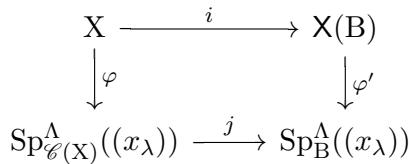
\includegraphics[keepaspectratio]{images/part001_f1662ccb.jpg}}

where \(\varphi\) and \(\varphi'\) are the mappings defined by the family \((x_{\lambda})_{\lambda \in \Lambda}\) (cf. no. 6 of I, p. 41), and \(i\) and \(j\) are the canonical injections. Then:

\begin{enumerate}
\def\labelenumi{\alph{enumi})}
\item
  The maps \(\varphi\) and \(\varphi'\) are homeomorphisms;
\item
  The simultaneous spectrum \(\mathrm{Sp}_{\mathrm{B}}^{\Lambda}((x_{\lambda}))\) is the polynomially convex hull of \(\mathrm{Sp}_{\mathcal{C}(\mathrm{X})}^{\Lambda}((x_{\lambda}))\) ;
\item
  The map \(\varphi\) maps \(\mathcal{C}(\mathrm{X})\) to \(\mathcal{C}(\mathrm{Sp}_{\mathcal{C}(\mathrm{X})}^{\Lambda}((x_{\lambda})))\) and B to \(\mathrm{P}(\mathrm{Sp}_{\mathcal{C}(\mathrm{X})}^{\Lambda}((x_{\lambda})))\) ;
\item
  The map \(\varphi^{\prime}\) maps \(\mathcal{G}_{\mathrm{B}}(\mathrm{B})\) to \(\mathrm{P}(\mathrm{Sp}_{\mathrm{B}}^{\Lambda}((x_{\lambda})))\) ;
\item
  The maps \(\varphi\) and \(\varphi'\) map \(\mathcal{G}_{\mathrm{B}}\) to the canonical isomorphism from \(\mathrm{P}(\mathrm{Sp}_{\mathcal{C}(\mathrm{X})}^{\Lambda}((x_{\lambda})))\) onto \(\mathrm{P}(\mathrm{Sp}_{\mathrm{B}}^{\Lambda}((x_{\lambda})))\) .
\end{enumerate}

The maps \(\varphi\) and \(\varphi'\) are continuous and surjective (I, no. 6, p.~41). The map \(\varphi'\) is a homeomorphism by assertion \(a\) ) of prop. 12 of I, p.~43, and \(i\) is injective, therefore \(\varphi\) is injective. Therefore \(\varphi\) and \(\varphi'\) are homeomorphisms.

Let \(X_{1} = \mathrm{Sp}_{\mathcal{C}(X)}^{\Lambda}((x_{\lambda}))\) . The polynomially convex hull of \(X_{1}\) is \(Y_{1} = \mathrm{Sp}_{\mathrm{B}}^{\Lambda}((x_{\lambda}))\) by prop. 14 of I, p.~46.

For every \(\lambda\in\Lambda\) , let \(z_{\lambda}\) be the corresponding coordinate function on \(\mathbf{C}^{\Lambda}\) . The map \(\varphi\) maps \(x_{\lambda}\) to \(z_{\lambda}|X_{1}\) , and \(\varphi'\) maps \(\mathcal{G}_{\mathrm{B}}(x_{\lambda})\) to \(z_{\lambda}|Y_{1}\) . Therefore \(\varphi\) maps B onto \(\mathrm{P}(X_{1})\) , and \(\varphi'\) maps \(\mathcal{G}_{\mathrm{B}}(B)\) onto \(\mathrm{P}(Y_{1})\) . Finally, \(\varphi\) and \(\varphi'\) map \(\mathcal{G}_{\mathrm{B}}\) to the canonical isomorphism from \(\mathrm{P}(X_{1})\) onto \(\mathrm{P}(Y_{1})\) .

COROLLARY 1. --- Let \(\Lambda\) be a set and X a compact subset of \(\mathbf{C}^{\Lambda}\) . We identify X with a subset of \(\mathsf{X}(\mathrm{P}(\mathrm{X}))\) (prop. 1 of I, p.~142, d)). Let \((z_{\lambda})_{\lambda \in \Lambda}\) be the family of coordinate functions on \(\mathbf{C}^{\Lambda}\) .

\begin{enumerate}
\def\labelenumi{\alph{enumi})}
\item
  The map \(\theta\) from \(\mathrm{X}(\mathrm{P}(\mathrm{X}))\) onto \(\mathrm{Sp}_{\mathrm{P}(\mathrm{X})}^{\Lambda}((z_{\lambda}))\) defined by the family \((z_{\lambda})\) is a homeomorphism from \(\mathrm{X}(\mathrm{P}(\mathrm{X}))\) onto the polynomially convex hull \(Y\) of \(X\). Its restriction to \(X\) is the identity map of \(X\) ;
\item
  For every function \(f \in \mathrm{P}(\mathrm{X})\) , the homeomorphism \(\theta\) transforms the extension \(\mathcal{G}_{\mathrm{P}(\mathrm{X})}(f)\) of \(f\) to \(\mathrm{X}(\mathrm{P}(\mathrm{X}))\) into an extension \(\widetilde{f}\) of \(f\) to \(\mathrm{Y}\) . The map \(f \mapsto \widetilde{f}\) is the canonical isomorphism from \(\mathrm{P}(\mathrm{X})\) onto \(\mathrm{P}(\mathrm{Y})\) .
\end{enumerate}

In prop. 4, take B = P(X) and \(x_{\lambda} = z_{\lambda}\) . Then \(\varphi\) becomes the identity map and \(\varphi'\) becomes the map \(\theta\) . The assertions of the corollary then reduce to those of loc. cit.

COROLLARY 2. --- Let \(\Lambda\) be a set and let \(X \subset \mathbf{C}^{\Lambda}\) be a compact set. If \(X\) is connected, then its polynomially convex hull is connected.

If X is connected, the only idempotents of \(\mathcal{C}(\mathrm{X})\) , hence of \(\mathrm{P}(\mathrm{X})\) , are 0 and 1 (cor. of prop. I, p.~79). Consequently, the space \(\mathrm{X}(\mathrm{P}(\mathrm{X}))\) is connected (loc. cit.); but this set is homeomorphic to the polynomially convex hull of X (cor. 1, a)).

\subsection{Continuous functions on a compact subset of C}

Lemma 1. --- Let X be a compact subset of the plane and let O be a bounded connected component of \(\mathbf{C} - \mathbf{X}\) . The boundary of O is contained in X.

The closure of the set O in C-X is equal to \(\overline{\mathrm{O}}\cap (\mathbf{C} - \mathbf{X})\) where \(\overline{\mathrm{O}}\) is its closure in C. Since O is a connected component of C-X, we therefore have \(\overline{\mathrm{O}}\cap (\mathbf{C} - \mathbf{X}) = \mathrm{O}\) , which indeed proves that \(\overline{\mathrm{O}} -\mathrm{O}\subset \mathrm{X}\) .

Let X be a compact subset of C. Let \(O_{\infty}\) be the unbounded connected component of \(\mathbf{C} - \mathbf{X}\) , and let \((\mathrm{O}_{i})_{i\in\mathrm{I}}\) be the family of bounded connected components of \(\mathbf{C} - \mathbf{X}\) , the sets \(O_{i}\) being pairwise distinct.

Let E be a subset of \(\mathbf{C} - \mathbf{X}\) . We denote by \(\mathrm{R}_{\mathrm{E}}(\mathrm{X})\) the closure in \(\mathcal{C}(\mathrm{X})\) of the set of functions \(f|\mathrm{X}\) , where \(f\) is a rational function on \(\mathbf{C}\) all of whose poles belong to E. The algebra \(\mathrm{R}_{\mathrm{E}}(\mathrm{X})\) is a unital Banach subalgebra of \(\mathcal{C}(\mathrm{X})\) which separates the points of X. Let z be the identity function on X. The full closed subalgebra of \(\mathrm{R}_{\mathrm{E}}(\mathrm{X})\) generated by z is equal to \(\mathrm{R}_{\mathrm{E}}(\mathrm{X})\) (lemma 2 of I, p.~6). The elements of \(\mathrm{R}_{\mathrm{E}}(\mathrm{X})\) are holomorphic in the interior of X.

In particular, we have \(\mathrm{R}_{\varnothing}(\mathrm{X})=\mathrm{P}(\mathrm{X})\) . We denote \(\mathrm{R}(\mathrm{X})=\mathrm{R}_{\mathbf{C}-\mathbf{X}}(\mathrm{X})\) . We denote by I(E) the set of elements \(i\in I\) such that \(E\cap O_{i}=\varnothing\) , and

\[
\mathrm{X} _ {\mathrm{E}} = \mathrm{X} \cup \Big (\bigcup_ {i \in \mathrm{I} (\mathrm{E})} \mathrm{O} _ {i} \Big).
\]

The set \(X_{E}\) is compact, since it is bounded and closed, its complement in \(\mathbf{C}\) being the union of the open \(O_{\infty}\) and open sets \(O_{i}\) that meet E.

PROPOSITION 5. --- With the above notation:

\begin{enumerate}
\def\labelenumi{\alph{enumi})}
\item
  The restriction map h of \(\mathrm{R}_{\mathrm{E}}(\mathrm{X}_{\mathrm{E}})\) into \(\mathrm{R}_{\mathrm{E}}(\mathrm{X})\) is an isometric isomorphism;
\item
  The algebra \(\mathrm{R}_{\mathrm{E}}(\mathrm{X}_{\mathrm{E}})\) is a full subalgebra of \(\mathcal{C}(\mathrm{X}_{\mathrm{E}})\) ;
\item
  Every character of \(\mathrm{R}_{\mathrm{E}}(\mathrm{X}_{\mathrm{E}})\) is of the form \(f \mapsto f(w)\) , where w is an element of \(X_{E}\) ;
\item
  The map \(\chi \mapsto \chi (z)\) is a homeomorphism from \(\mathsf{X}(\mathrm{R}_{\mathrm{E}}(\mathrm{X}))\) onto \(\mathrm{X}_{\mathrm{E}}\) ;
\item
  If E' is a subset of \(\mathbf{C} - \mathbf{X}\) , then we have \(\mathrm{R}_{\mathrm{E}}(\mathrm{X}) = \mathrm{R}_{\mathrm{E}'}(\mathrm{X})\) if and only if \(\mathrm{X}_{\mathrm{E}} = \mathrm{X}_{\mathrm{E}'}\) , which is also equivalent to \(\mathrm{I}(\mathrm{E}) = \mathrm{I}(\mathrm{E}')\) .
\end{enumerate}

The restriction map \(h\) of \(\mathrm{R}_{\mathrm{E}}(\mathrm{X}_{\mathrm{E}})\) into \(\mathrm{R}_{\mathrm{E}}(\mathrm{X})\) is a Banach algebra morphism such that \(\| h(f)\| \leqslant \| f\|\) for every function \(f\in \mathrm{R}_{\mathrm{E}}(\mathrm{X}_{\mathrm{E}})\) . Let \(f\in \mathrm{R}_{\mathrm{E}}(\mathrm{X}_{\mathrm{E}})\) . Let \(i\in \mathrm{I}(\mathrm{E})\) . Since \(f\) is holomorphic in a neighborhood of the bounded open set \(\mathrm{O}_i\) , the maximum principle (VAR, I, p.~29) implies that there exists an element \(z_0\) in the boundary of \(\mathrm{O}_i\) such that \(|f(z_0)| = \sup_{z\in \mathrm{O}_i}|f(z)|\) . Since the boundary of \(\mathrm{O}_i\) is contained in X (lemma 1), it follows that \(\sup_{z\in \mathrm{O}_i}|f(z)|\leqslant \| h(f)\|\) . Since this inequality holds for every \(i\in \mathrm{I}(\mathrm{E})\) , it results that \(\| f\| \leqslant \| h(f)\|\) . The morphism \(h\) is therefore isometric, and in particular injective. Let us now prove that it is surjective. Let \(g\in \mathrm{R}_{\mathrm{E}}(\mathrm{X})\) . There exists a sequence \((f_n)\) of rational functions whose poles belong to E which converges uniformly to \(g\) on X. The \(f_n|\mathrm{X}_{\mathrm{E}}\) are elements of \(\mathrm{R}_{\mathrm{E}}(\mathrm{X}_{\mathrm{E}})\) . Since \(h\) is isometric, the sequence \((f_n|\mathrm{X}_{\mathrm{E}})\) converges in \(\mathcal{C}(\mathrm{X}_{\mathrm{E}})\) . If \(f\) is its limit, we have \(f\in \mathrm{R}_{\mathrm{E}}(\mathrm{X}_{\mathrm{E}})\) and \(g = f|\mathrm{X} = h(f)\) . Hence \(a\) ) .

Let us prove assertion d). Apply prop. 3 of I, p.~144 to the algebra \(B = \mathrm{R}_{\mathrm{E}}(\mathrm{X})\) . Assertion b) of loc. cit. implies that the map which associates \(\chi(z)\) to \(\chi\) is a homeomorphism from \(\mathsf{X}(\mathrm{R}_{\mathrm{E}}(\mathrm{X}))\) onto \(\mathrm{Sp}_{\mathrm{R}_{\mathrm{E}}(\mathrm{X})}(z)\) . Let \(z_{\mathrm{E}}\) be the identity map of \(\mathrm{X}_{\mathrm{E}}\) . By loc. cit., a), we have \(\mathrm{Sp}_{\mathrm{R}_{\mathrm{E}}(\mathrm{X})}(z) = \mathrm{Sp}_{\mathrm{R}_{\mathrm{E}}(\mathrm{X}_{\mathrm{E}})}(z_{\mathrm{E}})\) . It therefore suffices to show that \(\mathrm{Sp}_{\mathrm{R}_{\mathrm{E}}(\mathrm{X}_{\mathrm{E}})}(z_{\mathrm{E}}) = \mathrm{X}_{\mathrm{E}}\) . The corollary of prop. 6 of I, p.~28 shows that \(\mathrm{Sp}_{\mathrm{R}_{\mathrm{E}}(\mathrm{X}_{\mathrm{E}})}(z_{\mathrm{E}})\) is the union of \(\mathrm{Sp}_{\mathcal{C}(\mathrm{X}_{\mathrm{E}})}(z_{\mathrm{E}}) = \mathrm{X}_{\mathrm{E}}\) and of certain bounded connected components of the complement of \(\mathrm{X}_{\mathrm{E}}\) . Let \(\mathrm{O}_{i}\) be one of the bounded connected components of the complement of \(\mathrm{X}_{\mathrm{E}}\) . The intersection \(\mathrm{E} \cap \mathrm{O}_{i}\) is therefore nonempty. Let \(\lambda \in \mathrm{E} \cap \mathrm{O}_{i}\) ; since \((\lambda - z_{\mathrm{E}})^{-1} \in \mathrm{R}_{\mathrm{E}}(\mathrm{X}_{\mathrm{E}})\) , we have \(\lambda \notin \mathrm{Sp}_{\mathrm{R}_{\mathrm{E}}(\mathrm{X}_{\mathrm{E}})}(z_{\mathrm{E}})\) . Thus, \(\mathrm{O}_{i}\) is not contained in \(\mathrm{Sp}_{\mathrm{R}_{\mathrm{E}}(\mathrm{X}_{\mathrm{E}})}(z_{\mathrm{E}})\) . This shows that \(\mathrm{Sp}_{\mathrm{R}_{\mathrm{E}}(\mathrm{X}_{\mathrm{E}})}(z_{\mathrm{E}}) = \mathrm{X}_{\mathrm{E}}\) .

This equality also implies that \(\mathrm{Sp}_{\mathrm{R}_{\mathrm{E}}(\mathrm{X}_{\mathrm{E}})}(z_{\mathrm{E}})=\mathrm{Sp}_{\mathcal{C}(\mathrm{X}_{\mathrm{E}})}(z_{\mathrm{E}})\) . This establishes condition (iii) of prop. 11 of I, p.~41, applied to the canonical injection of \(\mathrm{R}_{\mathrm{E}}(\mathrm{X}_{\mathrm{E}})\) into \(\mathcal{C}(\mathrm{X}_{\mathrm{E}})\) and to the element \(z_{\mathrm{E}}\) . Assertions b) and c) are the equivalent conditions (i) and (ii) of loc. cit.

Assertion \(d\) ) shows that \(\mathrm{X}_{\mathrm{E}} = \mathrm{X}_{\mathrm{E}'}\) if \(\mathrm{R}_{\mathrm{E}}(\mathrm{X}) = \mathrm{R}_{\mathrm{E}'}(\mathrm{X})\) . Conversely, suppose that \(\mathrm{X}_{\mathrm{E}} = \mathrm{X}_{\mathrm{E}'}\) . By replacing \(\mathrm{E}'\) by \(\mathrm{E} \cup \mathrm{E}'\) , we may assume that \(\mathrm{E} \subset \mathrm{E}'\) . According to \(b\) ), the algebra \(\mathrm{R}_{\mathrm{E}}(\mathrm{X}_{\mathrm{E}})\) is a full closed subalgebra of \(\mathcal{C}(\mathrm{X}_{\mathrm{E}})\) , and therefore also of \(\mathrm{R}_{\mathrm{E}'}(\mathrm{X}_{\mathrm{E}})\) . It contains \(z_{\mathrm{E}}\) , and hence \(\mathrm{R}_{\mathrm{E}}(\mathrm{X}_{\mathrm{E}}) = \mathrm{R}_{\mathrm{E}'}(\mathrm{X}_{\mathrm{E}})\) . Applying \(a\) ), we deduce that \(\mathrm{R}_{\mathrm{E}}(\mathrm{X}) = \mathrm{R}_{\mathrm{E}'}(\mathrm{X})\) . Finally, the equivalence of \(\mathrm{X}_{\mathrm{E}} = \mathrm{X}_{\mathrm{E}'}\) and \(\mathrm{I}(\mathrm{E}) = \mathrm{I}(\mathrm{E}')\) is a consequence of the definitions.

COROLLARY 1. --- The following conditions are equivalent:

\begin{enumerate}
\def\labelenumi{(\roman{enumi})}
\item
  The set E meets every bounded connected component of \(\mathbf{C} - \mathbf{X}\) ;
\item
  The map \(\chi \mapsto \chi (z)\) is a homeomorphism from \(\mathsf{X}(\mathrm{R}_{\mathrm{E}}(\mathrm{X}))\) onto \(\mathrm{X}\) ;
\item
  We have \(\mathrm{R_E(X)} = \mathrm{R(X)}\) .
\end{enumerate}

Let \(E' = \mathbf{C} - \mathbf{X}\) . Conditions (i), (ii), and (iii) are respectively equivalent to \(\mathrm{I}(\mathrm{E}) = \mathrm{I}(\mathrm{E}')\) , to \(\mathrm{X}_{\mathrm{E}} = \mathrm{X}_{\mathrm{E}'}\) (by prop. 5, d)) and to \(\mathrm{R}_{\mathrm{E}}(\mathrm{X}) = \mathrm{R}_{\mathrm{E}'}(\mathrm{X})\) . They are therefore equivalent to each other by prop. 5, e).

The following corollary makes the Runge theorem more precise (th. 3 of I, p.~69).

COROLLARY 2 (Runge's theorem). --- For every \(i \in I\) , let \(\lambda_{i}\) be a point of \(O_{i}\) . Let f be a complex function holomorphic in an open neighborhood of X. Then \(f|X\) is the uniform limit on X of restrictions of rational functions whose poles are among the \(\lambda_{i}\) .

With \(E = \{\lambda_{i}\}_{i \in I}\) , the hypothesis is condition (i) of Cor. 1. We therefore have \(\mathrm{R}_{\mathrm{E}}(\mathrm{X}) = \mathrm{R}(\mathrm{X})\) , and Th. 3 of I, p.~69 shows that \(\mathrm{R}(\mathrm{X}) = \mathcal{O}(\mathrm{X})\) .

\exercisesection{Spectra and Characters}


\begin{enumerate}
\def\labelenumi{\arabic{enumi})}
\item
  Let \((e_{1}, e_{2})\) be the canonical basis of \(R^{2}\) and let u be the element of A = \(\mathcal{L}(\mathbf{R}^{2})\) defined by \(u(e_{1}) = e_{2}\) , \(u(e_{2}) = -e_{1}\) . Prove that \(\mathrm{Sp}_{\mathrm{A}}(u) = \varnothing\) and \(\mathrm{Sp}_{\mathrm{A}}(u^{2}) = \{-1\}\) .
\item
  Let \(\mu\) be the Lebesgue measure on \([0,1]\) , H the Hilbert space \(\mathrm{L}_{\mathbf{C}}^{2}([0,1],\mu)\) , \(\mathrm{A} = \mathcal{L}(\mathrm{H})\) , and \(x \in \mathrm{A}\) the operator which transforms the function \(f(t)\) into the function \(tf(t)\) . Prove that \(\mathrm{Sp}_{\mathrm{A}}(x) = [0,1]\) , but that \(x\) has no eigenvalue.
\item
  \begin{enumerate}
  \def\labelenumii{\alph{enumii})}
  \tightlist
  \item
    Let H be a Hilbert space admitting a countable orthonormal basis \((e_{0}, e_{1}, e_{2}, \ldots)\) , and A = L(H). Let \(u \in \mathcal{L}(H)\) be such that \(u(e_{i}) = e_{i+1}\) for every i. Let \(u' \in \mathcal{L}(H)\) be such that \(u'(e_{i}) = e_{i-1}\) for \(i \geqslant 1\) and \(u'(e_{0}) = 0\) . We have \(u'u = 1\) but \(uu'(e_{0}) = 0\) , so that \(\mathrm{Sp}_{\mathrm{A}}(u'u) \neq \mathrm{Sp}_{\mathrm{A}}(uu')\) .
  \end{enumerate}
\end{enumerate}

\begin{enumerate}
\def\labelenumi{\alph{enumi})}
\setcounter{enumi}{1}
\tightlist
\item
  Let A be a unital Noetherian algebra over a commutative field. If \(x, y \in A\) , one has \(\mathrm{Sp}_{\mathrm{A}}(xy) = \mathrm{Sp}_{\mathrm{A}}(yx)\) (use exerc. 6 of A, VIII, p.~37).
\end{enumerate}

\begin{enumerate}
\def\labelenumi{\arabic{enumi})}
\setcounter{enumi}{3}
\tightlist
\item
  Let A be a commutative algebra over C, I an ideal of A, h the canonical injection of I into A, and S the set of \(\chi \in \mathsf{X}'(\mathsf{A})\) which vanish on I.
\end{enumerate}

\begin{enumerate}
\def\labelenumi{\alph{enumi})}
\item
  \(X'(h)\) is surjective.
\item
  \(\mathsf{X}^{\prime}(h)|(\mathsf{X}^{\prime}(\mathsf{A})-\mathsf{S})\) is a homeomorphism from \(\mathsf{X}^{\prime}(\mathsf{A})-\mathsf{S}\) onto \(\mathsf{X}(\mathsf{I})\) . (Let \(\chi_{0}\in\mathsf{X}^{\prime}(\mathsf{A})-\mathsf{S}\) . Let \(x_{1},\ldots,x_{n}\in\mathsf{A}\) , \(\varepsilon>0\) , and let V be the neighborhood of \(\chi_{0}\) in \(\mathsf{X}^{\prime}(\mathsf{A})\) defined by \(|(\chi-\chi_{0})(x_{i})|\leqslant\varepsilon,(i=1,\ldots,n)\) . Let \(u_{0}\in I\) be such that \(\chi_0(u_0) = 1\) . We have \(u_i = u_0x_i \in I\) . Then if \(|(\chi - \chi_0)(u_i)| \leqslant \delta\) ( \(i = 0, 1, \ldots, n\) ) with \(\delta\) small enough, we have \(\chi \in V\) .)
\end{enumerate}

\begin{enumerate}
\def\labelenumi{\arabic{enumi})}
\setcounter{enumi}{4}
\item
  In exerc. 4, take \(A = \mathbf{C}[X,Y]\) and \(I = AX\) . The space X(A) is identified with \(\mathbf{C}^2\) , S = \{0\} is identified with \(\{0\} \times \mathbf{C}\) . Let U be the set of \((\xi, \eta) \in \mathbf{C}^2\) such that \(|\xi| < e^{-|\eta|}\) . Prove that \(X'(h)(U)\) is not a neighborhood of 0 in \(X'(I)\) . Deduce that \(X'(I)\) does not identify with the quotient space of \(X'(A)\) by the equivalence relation defined by \(X'(h)\) . (On this subject, cf.~I, p.~169, exerc. 17.)
\item
  Let A be a commutative algebra over a field and let I be a maximal ideal of A. Prove that we have \(A^{2} \subset I\) with \(\dim(A/I) = 1\) or else that A/I is a field. (Apply to A/I exercise 3 of A, I, p.~153.) In particular, if \(A^{2} = A\) , every maximal ideal of A is regular.
\item
  Let A be a commutative algebra over a commutative field K, \(x \in A\) and \(\alpha \in K\) . The set of \(\chi \in \mathsf{X}(\mathsf{A})\) such that \((\mathcal{G}x)(\chi) = \alpha\) is closed for the Jacobson topology. (Reduce to the case where A has a unit element, then to the case where \(\alpha = 0\) .)
\end{enumerate}

¶ 8) Let A be an algebra, I a two-sided ideal of A, \(\mathrm{J}^{\mathrm{I}}(\mathrm{A})\) the set of primitive ideals of A that do not contain I, and \(\widehat{A}^{I}\) the set of irreducible representations \(\pi \in \widehat{A}\) such that \(\pi(I) \neq 0\) .

\begin{enumerate}
\def\labelenumi{\alph{enumi})}
\item
  If \(\pi \in \widehat{\mathrm{A}}^{\mathrm{I}}\) , one has \(\pi | \mathrm{I} \in \widehat{\mathrm{I}}\) (lemma 5, \(a\) ) of I, p.~12). If representations \(\pi\) and \(\pi' \in \widehat{\mathrm{A}}\) are such that \(\pi | \mathrm{I}\) and \(\pi'|\mathrm{I}\) are equivalent, then \(\pi\) and \(\pi'\) are equivalent. (One may assume that \(\pi(x) = \pi'(x)\) for all \(x \in \mathrm{I}\) . Then, for every \(y \in \mathrm{A}\) , \(\pi(y)\) and \(\pi'(y)\) coincide on \(\sum_{x \in \mathrm{I}} \operatorname{Im} \pi(x)\) , and this subspace is equal to the space of \(\pi\) .)
\item
  If \(\pi \in \widehat{\mathrm{I}}\) , \(\pi\) extends to an element of \(\widehat{\mathrm{A}}^{\mathrm{I}}\) . (Let R be a maximal regular left ideal of I. Let \(g\) be a right unit of I modulo R. Assuming that A admits a unit element, show that the relation \(\mathrm{AR} + \mathrm{A}(1 - g) = \mathrm{A}\) would entail \(g^2 \in \mathrm{R}\) . Therefore \(\mathrm{AR} + \mathrm{A}(1 - g)\) is contained in a maximal left ideal M of A. Prove that \(\mathrm{M} \cap \mathrm{I} = \mathrm{R}\) and \(\mathrm{M} + \mathrm{I} = \mathrm{A}\) .)
\item
  Deduce from a) and b) that the map \(I'\mapsto I'\cap I\) is a homeomorphism from \(\mathrm{J}^{\mathrm{I}}(\mathrm{A})\) onto \(\mathrm{J}(\mathrm{I})\) , and that the map \(\pi\mapsto\pi|I\) is a homeomorphism from \(\widehat{A}^{I}\) onto \(\widehat{I}\) .
\end{enumerate}
